\lhead{\emph{Dominio del problema}}
\chapter{Dominio del problema}

\begin{cabstract}
En el que se detalla la etapa de identificación de las características de la infraestructura donde el sistema se integrará, los diferentes usuarios que interactuarán con este y sus necesidades, y las propuestas de solución actuales relativas a la construcción de un sistema similar al planteado.
\end{cabstract}

La utilización de algoritmos distribuidos implica mejoras sustanciales en una gran cantidad de aplicaciones, incrementando la capacidad global de cómputo de un sistema mediante la unión de varios dispositivos que trabajan como una única entidad manteniendo simultáneamente un alto grado de independencia y una tolerancia global a fallos muy alta. Sin embargo, el coste de la adquisición, instalación y mantenimiento de dicho conjunto de nodos suele ser elevado. Además, los beneficios citados implican una mayor complejidad en el desarrollo de algoritmos que puedan aprovechar de forma óptima este tipo de sistemas. Varios factores como la sincronización y la comunicación entre partes, o errores tales como condiciones de carrera son mucho más comunes que en otro tipo de aplicaciones. Dichas circunstancias dificultan el desarrollo de este sistema y la comprensión de los fundamentos básicos de la Computación Distribuida, aspecto de relevancia para estudiantes de Ciencias de la Computación.

Si bien la mayoría de las aplicaciones en las que el paradigma de computación distribuida introduce mejoras suelen exigir una gran capacidad de cálculo, su desarrollo únicamente requiere un conjunto de instancias independientes de un \textit{software} (sistema operativo, contenedor de servicios\dots) con las que trabajar. Dicha característica implica que la utilización de nodos de precio reducido (o incluso equipos ya presentes en una infraestructura) para el diseño, análisis y evaluación de este tipo de algoritmos constituye una alternativa válida frente a sistemas de precio superior.

Sumada a dicha motivación existe el potencial aprovechamiento de este sistema como herramienta didáctica que facilite el aprendizaje de conceptos como el reparto de procesos, balance de carga o la compartición de recursos en asignaturas centradas en este tipo de computadores dentro de los planes de estudio de Ingeniería Informática o titulaciones similares.

En el presente proyecto se realiza un análisis de las diferentes alternativas que permitan satisfacer los objetivos definidos previamente como soporte a la toma de una decisión final.

\section{Definición del dominio del problema}

\subsection{Sistema actual: Infraestructura de la Facultad de Ciencias}
\label{dominioproblema:infraestructura}
El sistema se ubica en una Facultad universitaria con 1.463 alumnos, de los cuales 562 son estudiantes de titulaciones relacionadas con las Ciencias de la Computación \cite{uecusal:estudiantes}. Estas titulaciones cuentan con varias asignaturas relacionadas con el áreas de conocimiento Computación Distribuida, en particular \textbf{Arquitectura de Computadores} y \textbf{Sistemas Distribuidos} \cite{DIA15GuiaAcademica}. La Facultad cuenta con varias aulas y laboratorios de informática donde los alumnos disponen de las herramientas necesarias para realizar los ejercicios y prácticas asignadas. Dichos espacios permiten utilizar cualquier equipo como nodo, dado que se integran en la misma red, siendo factible la comunicación directa entre equipos situados en diferentes aulas o incluso edificios. Todos los equipos cuentan con una conexión de red cableada capaz de soportar teóricamente transferencias de hasta 100 Mb/s de forma bidireccional, compartiendo un mismo espacio de direcciones de red (no existen \textit{routers} entre diferentes secciones de este segmento de la red de la Universidad). La gestión de credenciales de autenticación se delega a un directorio \textbf{LDAP} (\textit{Lightweight Directory Access Protocol}) \cite{RFC4516-comment},y se cuenta con con un sistema de ficheros centralizado que permite acceder a la información de un usuario desde cualquier equipo, facilitando las tareas de replicación de la información entre nodos a través de los protocolos \textbf{NFS} y \textbf{Samba}. Todos estos datos han sido extraídos de diferentes entrevistas con el Administrador de la infraestructura.

La mayoría de las prácticas asignadas en las asignaturas de interés son desarrolladas en los lenguajes de programación \textbf{C} y \textbf{Java}, ya conocidos por la totalidad de los estudiantes gracias a asignaturas previamente cursadas.

\subsubsection{Problemas conocidos}

Si bien la infraestructura existente es capaz de proveer a los estudiantes de los recursos necesarios para la realización de los diferentes ejercicios, se identifican una serie de problemas:

\begin{itemize}
  \item Cada grupo de alumnos necesita tres estaciones de trabajo para poder realizar algunos de los ejercicios propuestos, y acceso físico a los mismos, consumiendo una gran cantidad de espacio.
  \item El servidor \textbf{NFS} constituye un ``cuello de botella'', pues todos los alumnos acceden a él de forma intensiva, causando una excesiva carga de trabajo por el gran número de peticiones al mismo.
  \item Existen una serie de problemas con las herramientas de desarrollo utilizadas actualmente, como la dificultad de configuración o la ubicación e identificación de recursos.
\end{itemize}

\subsubsection{Rendimiento}
\label{dominio:estadisticas}
%Pandora magic
Uno de los problemas actuales que la infraestructura presenta es la sobrecarga de los diferentes recursos centralizados, como son el servidor LDAP y el sistema de almacenamiento NFS/Samba.

\begin{figure}[H]
\centering
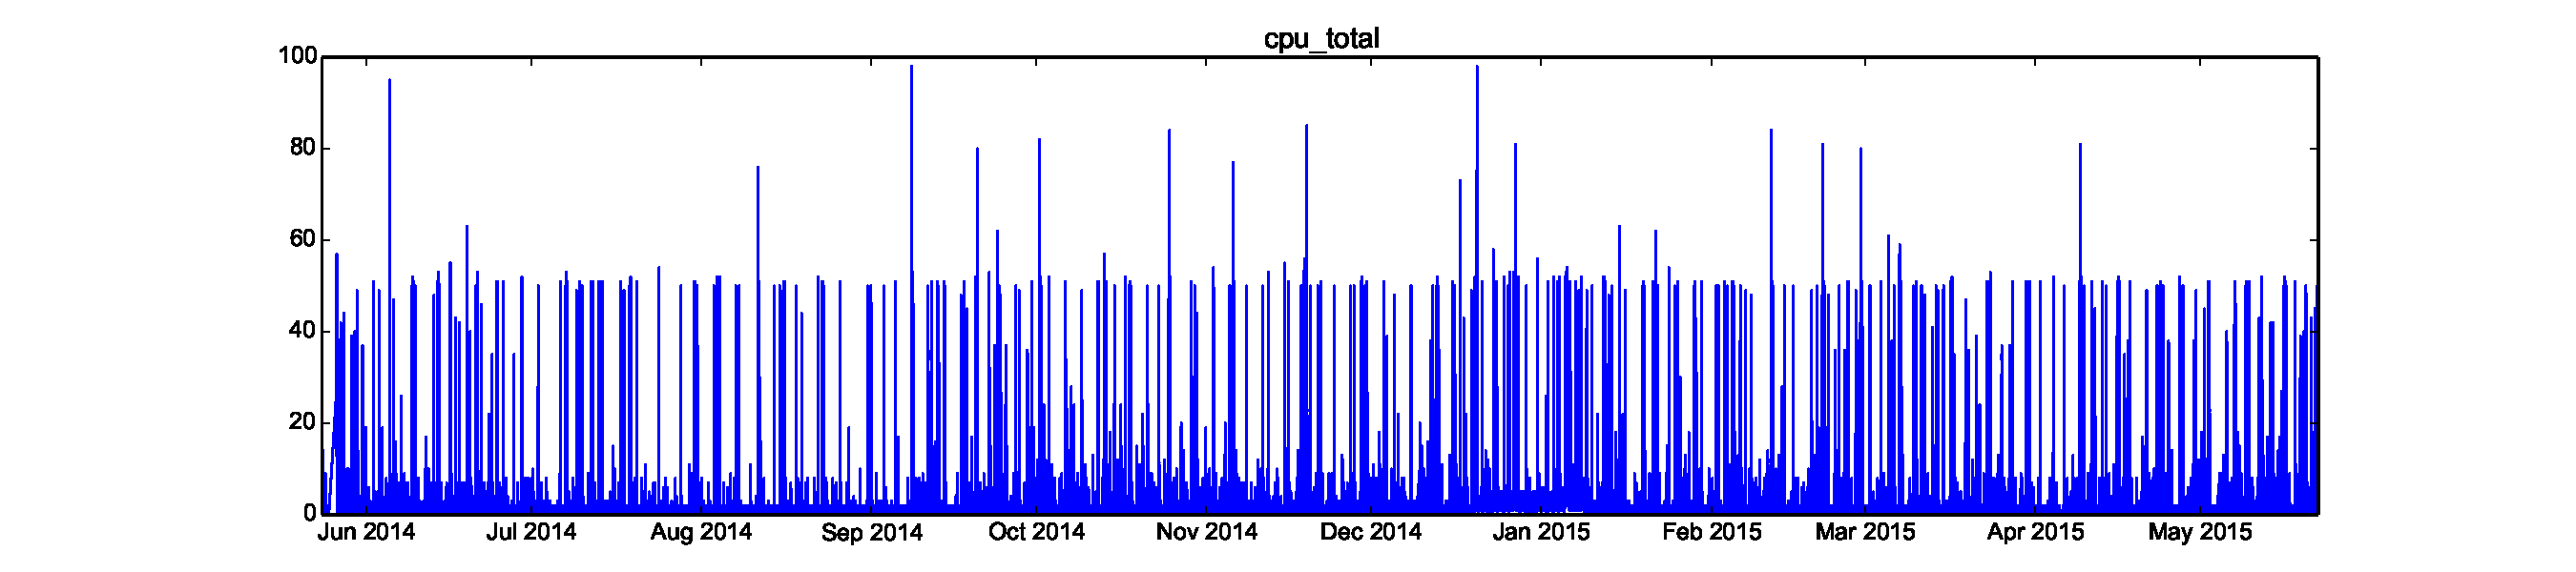
\includegraphics[width=\textwidth]{Chapters/Chapter4/Figures/data/cpu_total-2014-05-23_21:27:50-2015-05-22_13:41:46}
\caption{Porcentaje de CPU utilizada del servidor NFS}
\end{figure}

\begin{figure}[H]
\centering
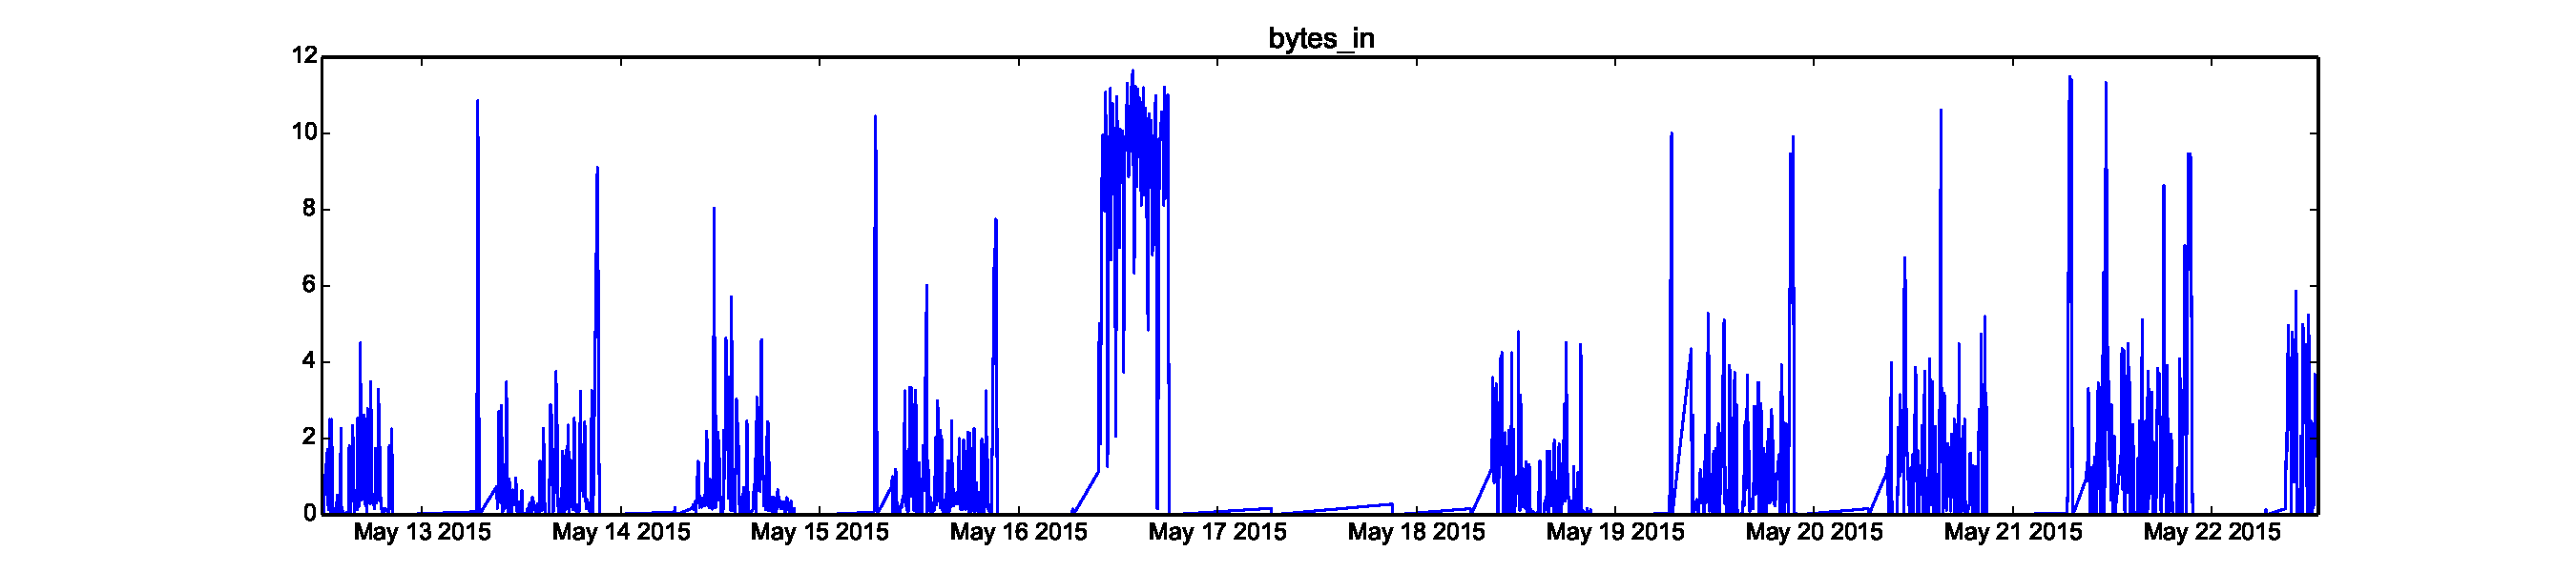
\includegraphics[width=\textwidth]{Chapters/Chapter4/Figures/data/bytes_in-2015-05-12_11:56:26-2015-05-22_12:51:08}
\caption{Datos de entrada al servidor durante un periodo de 10 días}.
\end{figure}

\begin{figure}[H]
\centering
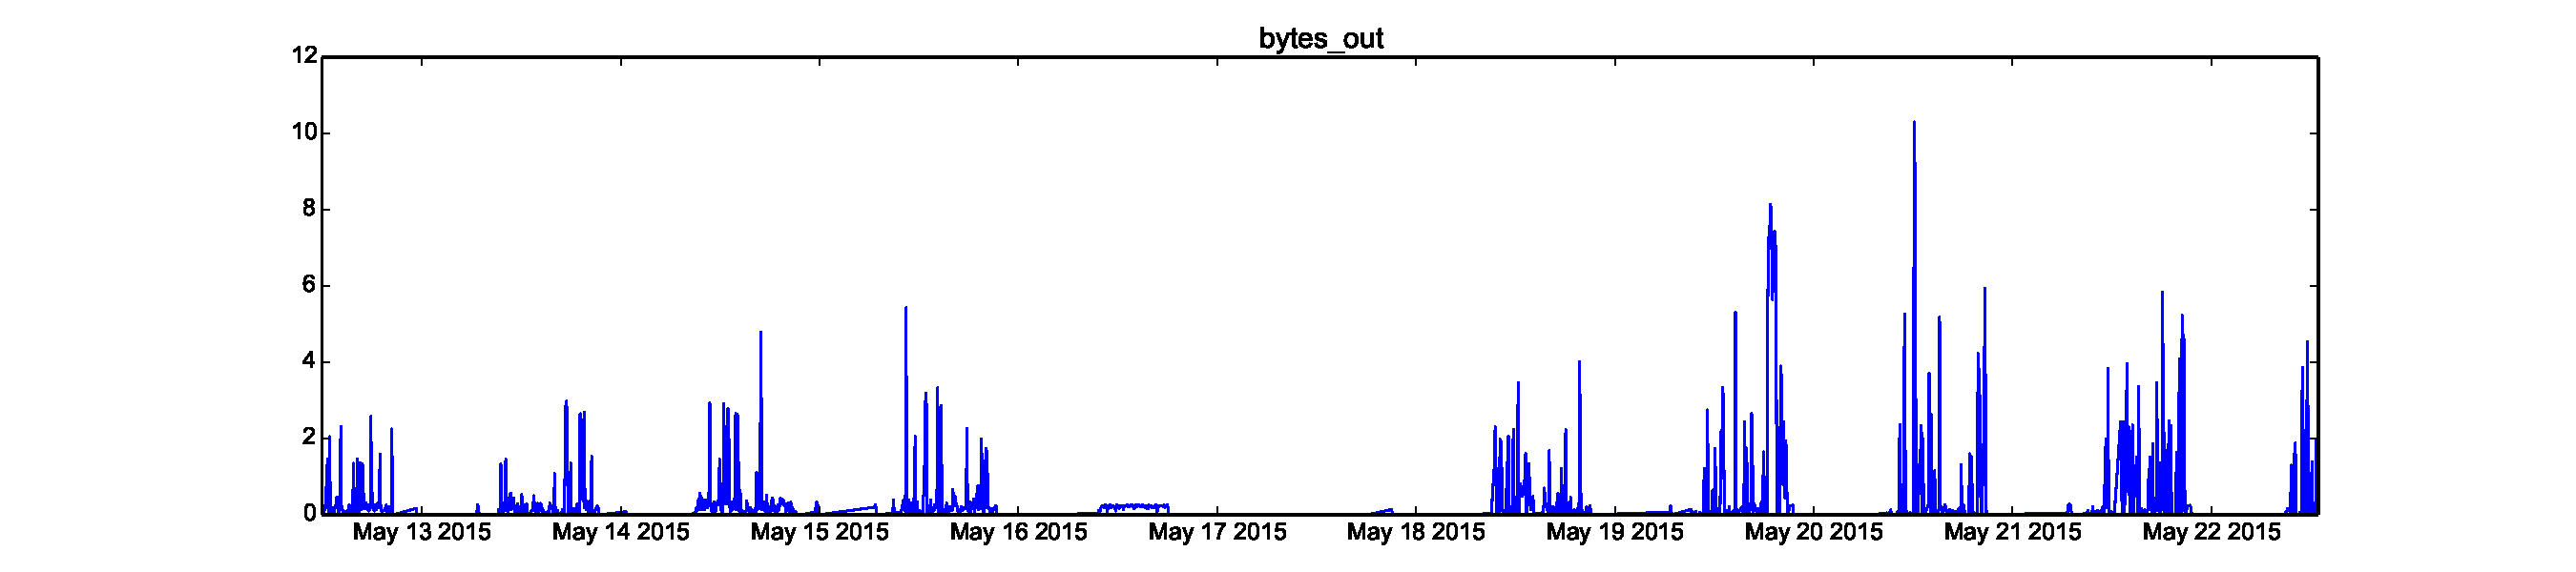
\includegraphics[width=\textwidth]{Chapters/Chapter4/Figures/data/bytes_out-2015-05-12_11:56:26-2015-05-22_12:56:12}
\caption{Datos de salida durante un periodo de 10 días}
\end{figure}

\section{Identificación de \textit{stakeholders}}

Un \textit{stakeholder} es cualquier grupo o individuo que afecta o es afectado por la consecución de los objetivos de un proyecto marcados por una organización, así como un particular interés en el devenir del mismo. Claros ejemplos de este tipo de entidades son los diferentes usuarios finales del sistema, potenciales clientes o el equipo de desarrollo, entre muchos otros.

En el proyecto en cuestión se identifican los siguientes \textit{stakeholders} y su motivación:

\begin{itemize}
  \item Equipo de desarrollo. Su motivación es la consecución de todos los objetivos marcados en el sistema. Dentro de este grupo existen dos categorías: los desarrolladores y los supervisores del proyecto.
  \item Estudiantes de tercer y cuarto curso del Grado en Ingeniería Informática, que podrán utilizar el sistema como herramienta didáctica.
  \item Profesores de las asignaturas Arquitectura de Computadores y Sistemas Distribuidos, que aprovecharán el sistema final en dichas asignaturas.
  \item Administradores del sistema, que deberán hacerse cargo del mantenimiento del sistema a largo plazo.
\end{itemize}

\subsection{Identificación de las necesidades de cada \textit{stakeholder}}

Basándose en la motivación de cada parte es posible definir las demandas de cada una de las partes. Otros mecanismos, como la realización de entrevistas u observaciones permiten complementan dicho proceso.

\subsubsection{Equipo de desarrollo}

\begin{itemize}
\item Acceso a diferentes recursos gestionados por la infraestructura.
\item Acceso a herramientas que permitan construir el \textit{software} y \textit{hardware} a desarrollar.
\end{itemize}

\subsubsection{Alumnos}

\begin{itemize}
  \item Entorno de trabajo intuitivo y documentado que agilice el desarrollo de sus prácticas.
  \item Posibilidad de observar los resultados de las ejecuciones de forma sencilla.
  \item Depuración sencilla.
  \item Facilidades para el despliegue de los diferentes ejecutables en todas las máquinas, así como el consumo de los servicios que estos implementen.
\end{itemize}

\subsubsection{Docentes}

\begin{itemize}
  \item Entorno versátil sobre el cual puedan llevarse a cabo la totalidad de las prácticas y ejercicios propuestos, aportando si es posible algún tipo de ventaja sobre el sistema en uso.
  \item Instalación y configuración simple.
\end{itemize}

\subsubsection{Administradores}

\begin{itemize}
  \item Sistema integrable en la infraestructura actual cuyo mantenimiento sea sencillo y cuyo enfoque garantice la escalabilidad y su durabilidad. Documentación extensa sobre el funcionamiento interno del sistema.
  \item Instalación y configuración simple.
  \item Mantenimiento sencillo.
\end{itemize}

\section{Propuestas para la búsqueda de necesidades}

\begin{itemize}
  \item Encuestas o entrevistas a todas las partes.
  \item Observación.
  \item Evaluación de la experiencia de uso en las diferentes etapas de desarrollo del sistema.
\end{itemize}

\section{Definición de objetivos}

\begin{table}[H]
\begin{tabular}{|p{2.5cm}|p{10cm}|}
\hline
\textbf{OBJ-1} &Creación de un sistema distribuido no jerárquico\\
\hline
\textbf{Versión} &1\\
\hline
\textbf{Autores} &Diego Martín\\
\hline
\textbf{Fuentes} &Análisis preliminar del sistema\\
\hline
\textbf{Descripción} &El sistema a crear reducirá el número de ``cuellos de botella'' e interdependencias entre componentes mediante la distribución de recursos sin coordinador.\\
\hline
\textbf{Subobjetivos} &\\
\hline
\textbf{Importancia} &Alta\\
\hline
\textbf{Urgencia} &Alta\\
\hline
\textbf{Estado} &Completo\\
\hline
\textbf{Estabilidad} &Estable\\
\hline
\textbf{Comentarios} &\\
\hline
\end{tabular}
\caption{OBJ-1: Creación de un sistema distribuido no jerárquico}
\end{table}

\begin{table}[H]
\begin{tabular}{|p{2.5cm}|p{10cm}|}
\hline
\textbf{OBJ-2} &Integración\\
\hline
\textbf{Versión} &1\\
\hline
\textbf{Autores} &Diego Martín\\
\hline
\textbf{Fuentes} &Análisis preliminar\\
\hline
\textbf{Descripción} &El sistema creado deberá ser creado para que su integración con la infraestructura presente en la Facultad de Ciencias sea trivial.\\
\hline
\textbf{Subobjetivos} &\\
\hline
\textbf{Importancia} &Alta\\
\hline
\textbf{Urgencia} &Alta\\
\hline
\textbf{Estado} &Completo\\
\hline
\textbf{Estabilidad} &Estable\\
\hline
\textbf{Comentarios} &\\
\hline
\end{tabular}
\caption{OBJ-2: Integración}
\end{table}

\begin{table}[H]
\begin{tabular}{|p{2.5cm}|p{10cm}|}
\hline
\textbf{OBJ-3} &Evaluación\\
\hline
\textbf{Versión} &1\\
\hline
\textbf{Autores} &Diego Martín\\
\hline
\textbf{Fuentes} &Análisis preliminar del sistema\\
\hline
\textbf{Descripción} &Se realizarán diferentes evaluaciones técnicas y de usuario de los diferentes aspectos del desarrollo, con el objetivo de verificar la integración del sistema en una organización\\
\hline
\textbf{Subobjetivos} &\\
\hline
\textbf{Importancia} &\\
\hline
\textbf{Urgencia} &\\
\hline
\textbf{Estado} &\\
\hline
\textbf{Estabilidad} &\\
\hline
\textbf{Comentarios} &\\
\hline
\end{tabular}
\caption{OBJ-3: Evaluación}
\end{table}

\begin{table}[H]
\begin{tabular}{|p{2.5cm}|p{10cm}|}
\hline
\textbf{OBJ-4} &Estudio comparativo\\
\hline
\textbf{Versión} &1\\
\hline
\textbf{Autores} &Diego Martín, Rodrigo Santamaría\\
\hline
\textbf{Fuentes} &Reuniones de equipo\\
\hline
\textbf{Descripción} &Junto al desarrollo y evaluación de los productos a crear se deberá realizar un estudio comparativo de todas las soluciones propuestas\\
\hline
\textbf{Subobjetivos} &\\
\hline
\textbf{Importancia} &Alta\\
\hline
\textbf{Urgencia} &Alta\\
\hline
\textbf{Estado} &Completo\\
\hline
\textbf{Estabilidad} &Estable\\
\hline
\textbf{Comentarios} &\\
\hline
\end{tabular}
\caption{OBJ-4: Estudio comparativo}
\end{table}

\section{Identificación de requisitos}

Los requisitos relativos a cada herramienta son detallados en el anexo correspondientes (ver apéndice \ref{listaanexos}), sirviendo esta sección para aportar una perspectiva a alto nivel de los diferentes requisitos. Es por ello que los requisitos funcionales, vinculados fuertemente a la interacción del usuario con el sistema, son recogidos únicamente en este documento.

\subsection{Requisitos de almacenamiento de la información}

Se identifican los siguientes requisitos de información a alto nivel.

\begin{table}[H]
\centering
\begin{tabular}{|p{3.5cm}|p{10cm}|}
\hline
\textbf{IRQ-1} & Gestión de usuarios\\
\hline
\textbf{Versión} & 1.1\\
\hline
\textbf{Autores} &Diego Martín\\
\hline
\textbf{Fuentes} & Análisis preliminar del sistema. Reuniones de equipo.\\
\hline
\textbf{Objetivos asociados} & \citationneeded[TODO]\\
\hline
\textbf{Requisitos asociados} & \citationneeded[TODO]\\
\hline
\textbf{Descripción} & El sistema deberá consultar una fuente de datos (bien gestionada por el mismo o mantenida por un tercero) para realizar todas las operaciones de autenticación de los usuarios.\\
\hline
\textbf{Datos específicos} & Los propios de un sistema UNIX (UID, GID, nombre de usuario, grupos, directorio \texttt{\$HOME}).\\
\hline
\textbf{Tiempo de vida} & Permanente\\
\hline
\textbf{Ocurrencias simultáneas} & Se plantea la existencia de una única fuente de datos, consultada tantas veces como un usuario inicie sesión o realice cualquier otra operación en la que esta información deba ser verificada.\\
\hline
\textbf{Importancia} & Alta\\
\hline
\textbf{Urgencia} & Alta\\
\hline
\textbf{Estado} & Completo\\
\hline
\textbf{Estabilidad} & Estable\\
\hline
\textbf{Comentarios} & La versión 1.1 considera una fuente de datos de un tercero para la gestión de los usuarios\\
\hline
\end{tabular}
\caption{IRQ-1: Gestión de usuarios}
\end{table}

\begin{table}[H]
\centering
\begin{tabular}{|p{3.5cm}|p{10cm}|}
\hline
\textbf{IRQ-2} & \textit{Logs} del sistema\\
\hline
\textbf{Versión} & 1\\
\hline
\textbf{Autores} &Diego Martín\\
\hline
\textbf{Fuentes} & Análisis preliminar del sistema. Reuniones de equipo.\\
\hline
\textbf{Objetivos asociados} & \citationneeded[TODO]\\
\hline
\textbf{Requisitos asociados} & \citationneeded[TODO] \\
\hline
\textbf{Descripción} & Se deberán gestionar diferentes ficheros que sirvan como registro de todas las operaciones realizadas por el sistema con el objetivo de poder realizar operaciones de análisis o detección de errores posteriormente.\\
\hline
\textbf{Datos específicos} & Operaciones realizadas en las diferentes herramientas, incluyendo parámetros de operación, usuarios, resultados, condiciones irregulares\dots\\
\hline
\textbf{Tiempo de vida} & Se mantendrán estos archivos de forma permanente.\\
\hline
\textbf{Ocurrencias simultáneas} & Se plantea el uso de un fichero por cada aplicación.\\
\hline
\textbf{Importancia} &Alta\\
\hline
\textbf{Urgencia} &Media\\
\hline
\textbf{Estado} &Completo\\
\hline
\textbf{Estabilidad} &Estable\\
\hline
\textbf{Comentarios} &\\
\hline
\end{tabular}
\caption{IRQ-2: \textit{Logs} del sistema}
\end{table}

\begin{table}[H]
\centering
\begin{tabular}{|p{3.5cm}|p{10cm}|}
\hline
\textbf{IRQ-3} &Ficheros de configuración\\
\hline
\textbf{Versión} & 1\\
\hline
\textbf{Autores} &Diego Martín\\
\hline
\textbf{Fuentes} & Etapas de desarrollo\\
\hline
\textbf{Objetivos asociados} &\citationneeded[TODO]\\
\hline
\textbf{Requisitos asociados} &\citationneeded[TODO]\\
\hline
\textbf{Descripción} &La configuración de todas las aplicaciones se realizará a través de ficheros que incluyan todos los parámetros de interés. \\
\hline
\textbf{Datos específicos} &Cualquier valor modificable que altere el comportamiento de un programa (puerto de operación, directorios auxiliares\dots\\
\hline
\textbf{Tiempo de vida} &Permanente\\
\hline
\textbf{Ocurrencias simultáneas} &Se plantea el uso de un fichero por cada aplicación.\\
\hline
\textbf{Importancia} &Alta\\
\hline
\textbf{Urgencia} &Media\\
\hline
\textbf{Estado} &Completo\\
\hline
\textbf{Estabilidad} &Estable\\
\hline
\textbf{Comentarios} &\\
\hline
\end{tabular}
\caption{IRQ-3: Ficheros de configuración}
\end{table}

\begin{table}[H]
\centering
\begin{tabular}{|p{3.5cm}|p{10cm}|}
\hline
\textbf{IRQ-4} &Información aportada por los usuarios y de gestión\\
\hline
\textbf{Versión} & 1\\
\hline
\textbf{Autores} &Diego Martín\\
\hline
\textbf{Fuentes} & Fases de desarrollo del sistema\\
\hline
\textbf{Objetivos asociados} &\citationneeded[TODO]\\
\hline
\textbf{Requisitos asociados} &\citationneeded[TODO]\\
\hline
\textbf{Descripción} &Se utilizarán diferentes gestores de bases de datos para el almacenamiento de diferentes datos manejados por el sistema con el objetivo de facilitar el acceso a los mismos y su persistencia.\\
\hline
\textbf{Datos específicos} &Se plantea el almacenamiento de información aportada por el usuario, datos internos del sistema, etcétera\\
\hline
\textbf{Tiempo de vida} &Generalmente, los datos serán almacenados hasta que no se consideren de utilidad o un usuario o administrador decida eliminarlos.\\
\hline
\textbf{Ocurrencias simultáneas} &Se plantea el uso de una base de datos para cada tarea.\\
\hline
\textbf{Importancia} &Media\\
\hline
\textbf{Urgencia} &Media\\
\hline
\textbf{Estado} &Completo\\
\hline
\textbf{Estabilidad} &Estable\\
\hline
\textbf{Comentarios} &\\
\hline
\end{tabular}
\caption{IRQ-4: Información aportada por los usuarios y de gestión}
\end{table}


% \begin{comment}
% For future use
% \begin{table}[H]
% \begin{tabular}{|p{3.5cm}|p{10cm}|}
% \hline
% \textbf{IRQ-} &\\
% \hline
% \textbf{Versión} &\\
% \hline
% \textbf{Fuentes} &\\
% \hline
% \textbf{Objetivos asociados} &\\
% \hline
% \textbf{Requisitos asociados} &\\
% \hline
% \textbf{Descripción} &\\
% \hline
% \textbf{Datos específicos} &\\
% \hline
% \textbf{Tiempo de vida} &\\
% \hline
% \textbf{Ocurrencias simultáneas} &\\
% \hline
% \textbf{Importancia} &\\
% \hline
% \textbf{Urgencia} &\\
% \hline
% \textbf{Estado} &\\
% \hline
% \textbf{Estabilidad} &\\
% \hline
% \textbf{Comentarios} &\\
% \hline
% \end{tabular}
% \end{table}
% \end{comment}


\subsection{Identificación de requisitos no funcionales}

\begin{table}[H]
\centering
\begin{tabular}{|p{3.5cm}|p{10cm}|}
\hline
\textbf{NFR-1} &Mantenimiento y robustez\\
\hline
\textbf{Versión} &1\\
\hline
\textbf{Autores} & Diego Martín\\
\hline
\textbf{Fuentes} & Análisis preliminar del sistema\\
\hline
\textbf{Objetivos asociados} &\citationneeded[TODO]\\
\hline
\textbf{Requisitos asociados} &\citationneeded[TODO]\\
\hline
\textbf{Descripción} &El \textit{software} debe ser mantenible y robusto, siendo dicha robustez garantizada mediante el uso de \textit{software} utilizado por una base de usuarios significativa, una arquitectura conocida, pruebas realizadas sobre él o un equipo de desarrollo en activo, entre otras.\\
\hline
\textbf{Importancia} &Alta\\
\hline
\textbf{Urgencia} &Alta\\
\hline
\textbf{Estado} &Completo\\
\hline
\textbf{Estabilidad} &Estable\\
\hline
\textbf{Comentarios} &\\
\hline
\end{tabular}
\caption{NFR-1: Mantenimiento y robustez}
\end{table}

\begin{table}[H]
\centering
\begin{tabular}{|p{3.5cm}|p{10cm}|}
\hline
\textbf{NFR-2} &Coste de desarrollo\\
\hline
\textbf{Versión} &1\\
\hline
\textbf{Autores} & Diego Martín\\
\hline
\textbf{Fuentes} &Administración de la organización\\
\hline
\textbf{Objetivos asociados} &\citationneeded[TODO]\\
\hline
\textbf{Requisitos asociados} &\citationneeded[TODO]\\
\hline
\textbf{Descripción} &El coste de desarrollo no debe superar un total de 400 €.\\
\hline
\textbf{Importancia} &Alta\\
\hline
\textbf{Urgencia} &Alta\\
\hline
\textbf{Estado} &Completo\\
\hline
\textbf{Estabilidad} &Estable\\
\hline
\textbf{Comentarios} &\\
\hline
\end{tabular}
\caption{NFR-2: Coste de desarrollo}
\end{table}

\begin{table}[H]
\centering
\begin{tabular}{|p{3.5cm}|p{10cm}|}
\hline
\textbf{NFR-3} &Definición de los protocolos de comunicación\\
\hline
\textbf{Versión} &1\\
\hline
\textbf{Autores} & Diego Martín\\
\hline
\textbf{Fuentes} &Análisis preliminar\\
\hline
\textbf{Objetivos asociados} &\citationneeded[TODO]\\
\hline
\textbf{Requisitos asociados} &\citationneeded[TODO]\\
\hline
\textbf{Descripción} &Los diferentes protocolos utilizados o creados para el sistema deben ser públicos y extensibles a diferentes paradigmas de utilización y tecnologías que los implementen.\\
\hline
\textbf{Importancia} &Alta\\
\hline
\textbf{Urgencia} &Alta\\
\hline
\textbf{Estado} &Completo\\
\hline
\textbf{Estabilidad} &Estable\\
\hline
\textbf{Comentarios} &\\
\hline
\end{tabular}
\caption{NFR-3: Definición de los protocolos de comunicación}
\end{table}

\begin{table}[H]
\centering
\begin{tabular}{|p{3.5cm}|p{10cm}|}
\hline
\textbf{NFR-4} &Transparencia\\
\hline
\textbf{Versión} &1\\
\hline
\textbf{Autores} & Diego Martín\\
\hline
\textbf{Fuentes} &Análisis preliminar\\
\hline
\textbf{Objetivos asociados} &\citationneeded[TODO]\\
\hline
\textbf{Requisitos asociados} &\citationneeded[TODO]\\
\hline
\textbf{Descripción} &El sistema deberá cumplir todas las transparencias definidas en \ref{transparencias} en todas aquellas ocasiones en las que no se comprometa el funcionamiento del sistema.\\
\hline
\textbf{Importancia} &Media\\
\hline
\textbf{Urgencia} &Media\\
\hline
\textbf{Estado} &Completo\\
\hline
\textbf{Estabilidad} &Estable\\
\hline
\textbf{Comentarios} &\\
\hline
\end{tabular}
\caption{NFR-4: Transparencia}
\end{table}

\begin{table}[H]
\centering
\begin{tabular}{|p{3.5cm}|p{10cm}|}
\hline
\textbf{NFR-5} &Compatibilidad con prácticas y otros ejercicios didácticos\\
\hline
\textbf{Versión} &1\\
\hline
\textbf{Autores} & Diego Martín\\
\hline
\textbf{Fuentes} &Reuniones de equipo\\
\hline
\textbf{Objetivos asociados} &\citationneeded[TODO]\\
\hline
\textbf{Requisitos asociados} &\citationneeded[TODO]\\
\hline
\textbf{Descripción} &El sistema deberá ser compatible los ejercicios desarrollados en las asignaturas \textbf{Arquitectura de Computadores} y en especial \textbf{Sistemas distribuidos}\\
\hline
\textbf{Importancia} &Alta\\
\hline
\textbf{Urgencia} &Media\\
\hline
\textbf{Estado} &Completo\\
\hline
\textbf{Estabilidad} &Estable\\
\hline
\textbf{Comentarios} &\\
\hline
\end{tabular}
\caption{NFR-5: Compatibilidad con prácticas y otros ejercicios didácticos}
\end{table}

% \begin{comment}
% For future use
% \begin{table}[H]
% \begin{tabular}{|p{3.5cm}|p{10cm}|}
% \hline
% \textbf{NFR-} &\\
% \hline
% \textbf{Versión} &\\
% \hline
% \textbf{Fuentes} &\\
% \hline
% \textbf{Objetivos asociados} &\\
% \hline
% \textbf{Requisitos asociados} &\\
% \hline
% \textbf{Descripción} &\\
% \hline
% \textbf{Importancia} &\\
% \hline
% \textbf{Urgencia} &\\
% \hline
% \textbf{Estado} &\\
% \hline
% \textbf{Estabilidad} &\\
% \hline
% \textbf{Comentarios} &\\
% \hline
% \end{tabular}
% \end{table}
% \end{comment}


\section{Situación actual (\textit{state of the art})}
\label{stateoftheart}
En esta sección se definen diferentes enfoques ya aplicados a soluciones a problemas similares al planteado anteriormente.

\subsection{Computadores de placa única}

El uso de computadores de prestaciones reducidas como componentes de un sistema distribuido ha experimentado un gran crecimiento en los últimos años debido a la popularización y el abaratamiento de este tipo de dispositivos, existiendo gran cantidad de fabricantes y proveedores de \textit{software} para los mismos.

Los computadores de placa única (\textit{Single-Board Computers}) son máquinas de generalmente bajas prestaciones que aglutinan todos los componentes necesarios para su funcionamiento en un único circuito impreso. Suelen tener un coste bajo y una relación rendimiento/coste elevada. Su versatilidad y precio reducido han propiciado su uso como herramienta para el estudio y creación de sistemas distribuidos con un gran rango de propósitos diferentes.

\subsubsection{RPiCluster (Joshua Kiepert)}

Joshua Kiepert, estudiante de doctorado en la universidad Boise State, crea este sistema utilizando 33 computadores \textbf{Raspberry Pi B}, con el objetivo de utilizarlo como herramienta de pruebas que sirva de alternativa al supercomputador con el que su universidad cuenta\cite{joshuarpicluster} y sobre el que trabaja de forma rutinaria, con el objetivo de poder continuar su trabajo en periodos de mantenimiento, cierre del centro, etcétera. El sistema está diseñado para utilizar la \textit{Message Passing Interface} como mecanismo de comunicación y coordinación (siguiendo un esquema maestro-esclavo) y además utilizar los diferentes puertos de las placas (GPIO, I\textsuperscript{2}C, SPI, UART), puertos generalmente ausentes en computadores convencionales. Utiliza además un sistema \textbf{NFS} (\textit{Network File Storage}) para compartir datos entre todos los nodos, y un \textit{router} dedicado para la interconexión. El sistema se completa con un ordenador portátil \textbf{Chromebook} con el mismo sistema operativo que los nodos del sistema, (\textbf{Arch Linux}), que actúa como nodo coordinador. La estructura incluye el conjunto de nodos esclavos y coordinador, dos fuentes de alimentación y un mecanismo de refrigeración, así como un mecanismo de distribución de la energía (diseñado por Kiepert) y de gestión de los diodos LED que incluye cada nodo y que son utilizados como elemento estético y mecanismo de análisis visual del comportamiento de los algoritmos ejecutados\footnote{Vídeo del sistema en ejecución: \href{https://www.youtube.com/watch?v=i_r3z1jYHAc}{youtube.com/watch?v=i\_r3z1jYHAc}}.

%TODO: http://www.zdnet.com/article/build-your-own-supercomputer-out-of-raspberry-pi-boards/

\begin{figure}[H]
  \centering
  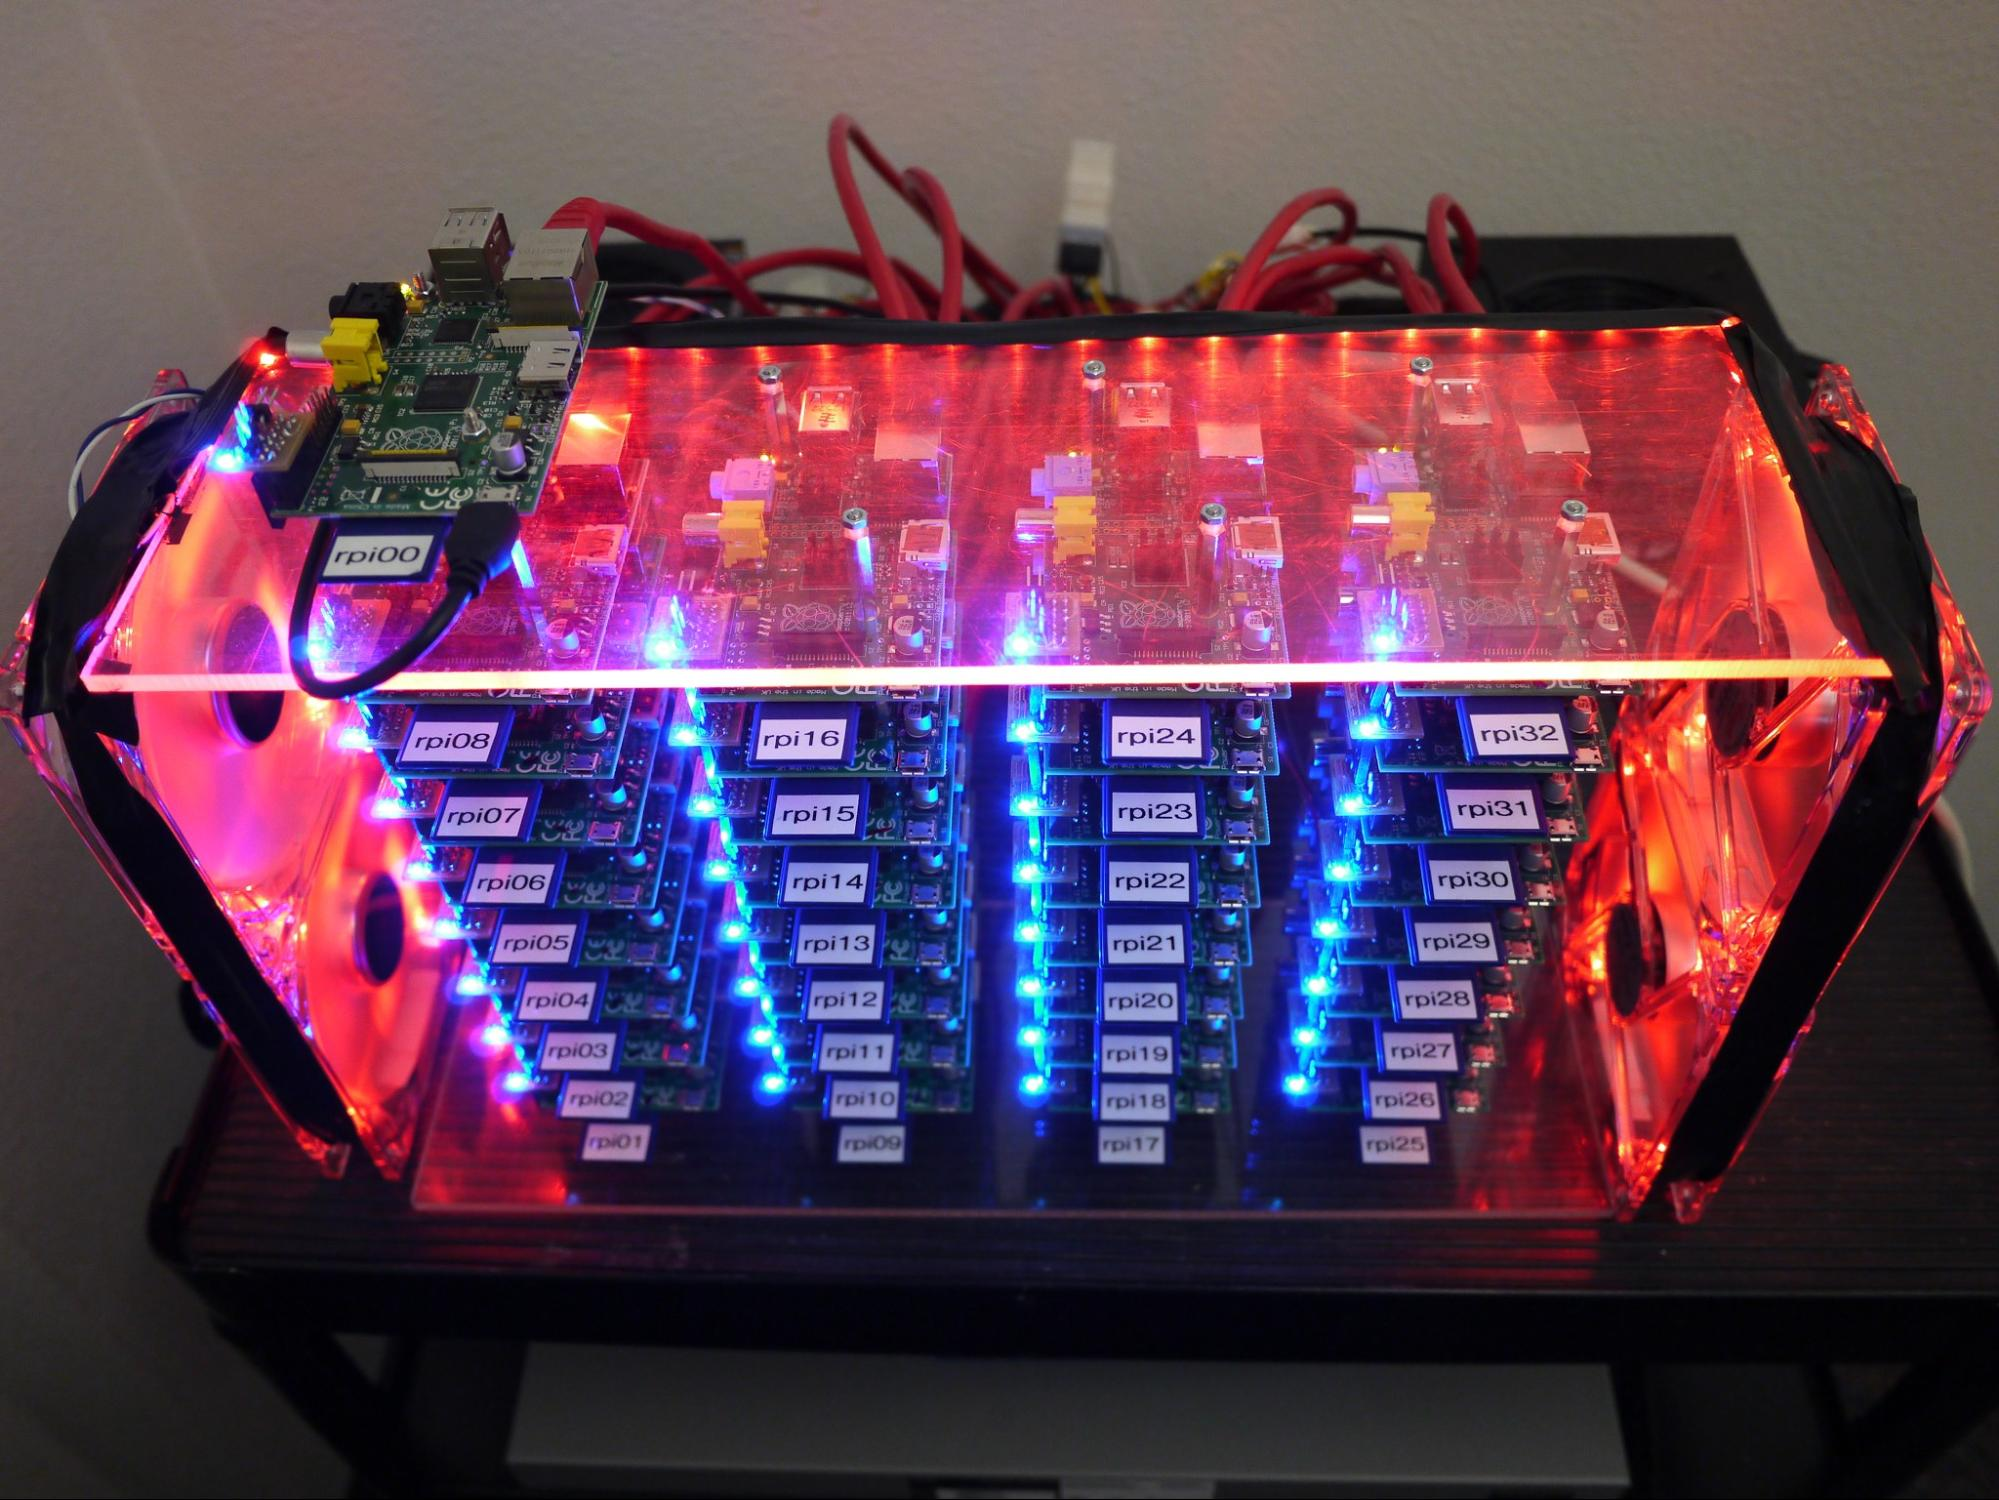
\includegraphics[width=0.36\textwidth]{Chapter4/Figures/kiepert-main}
  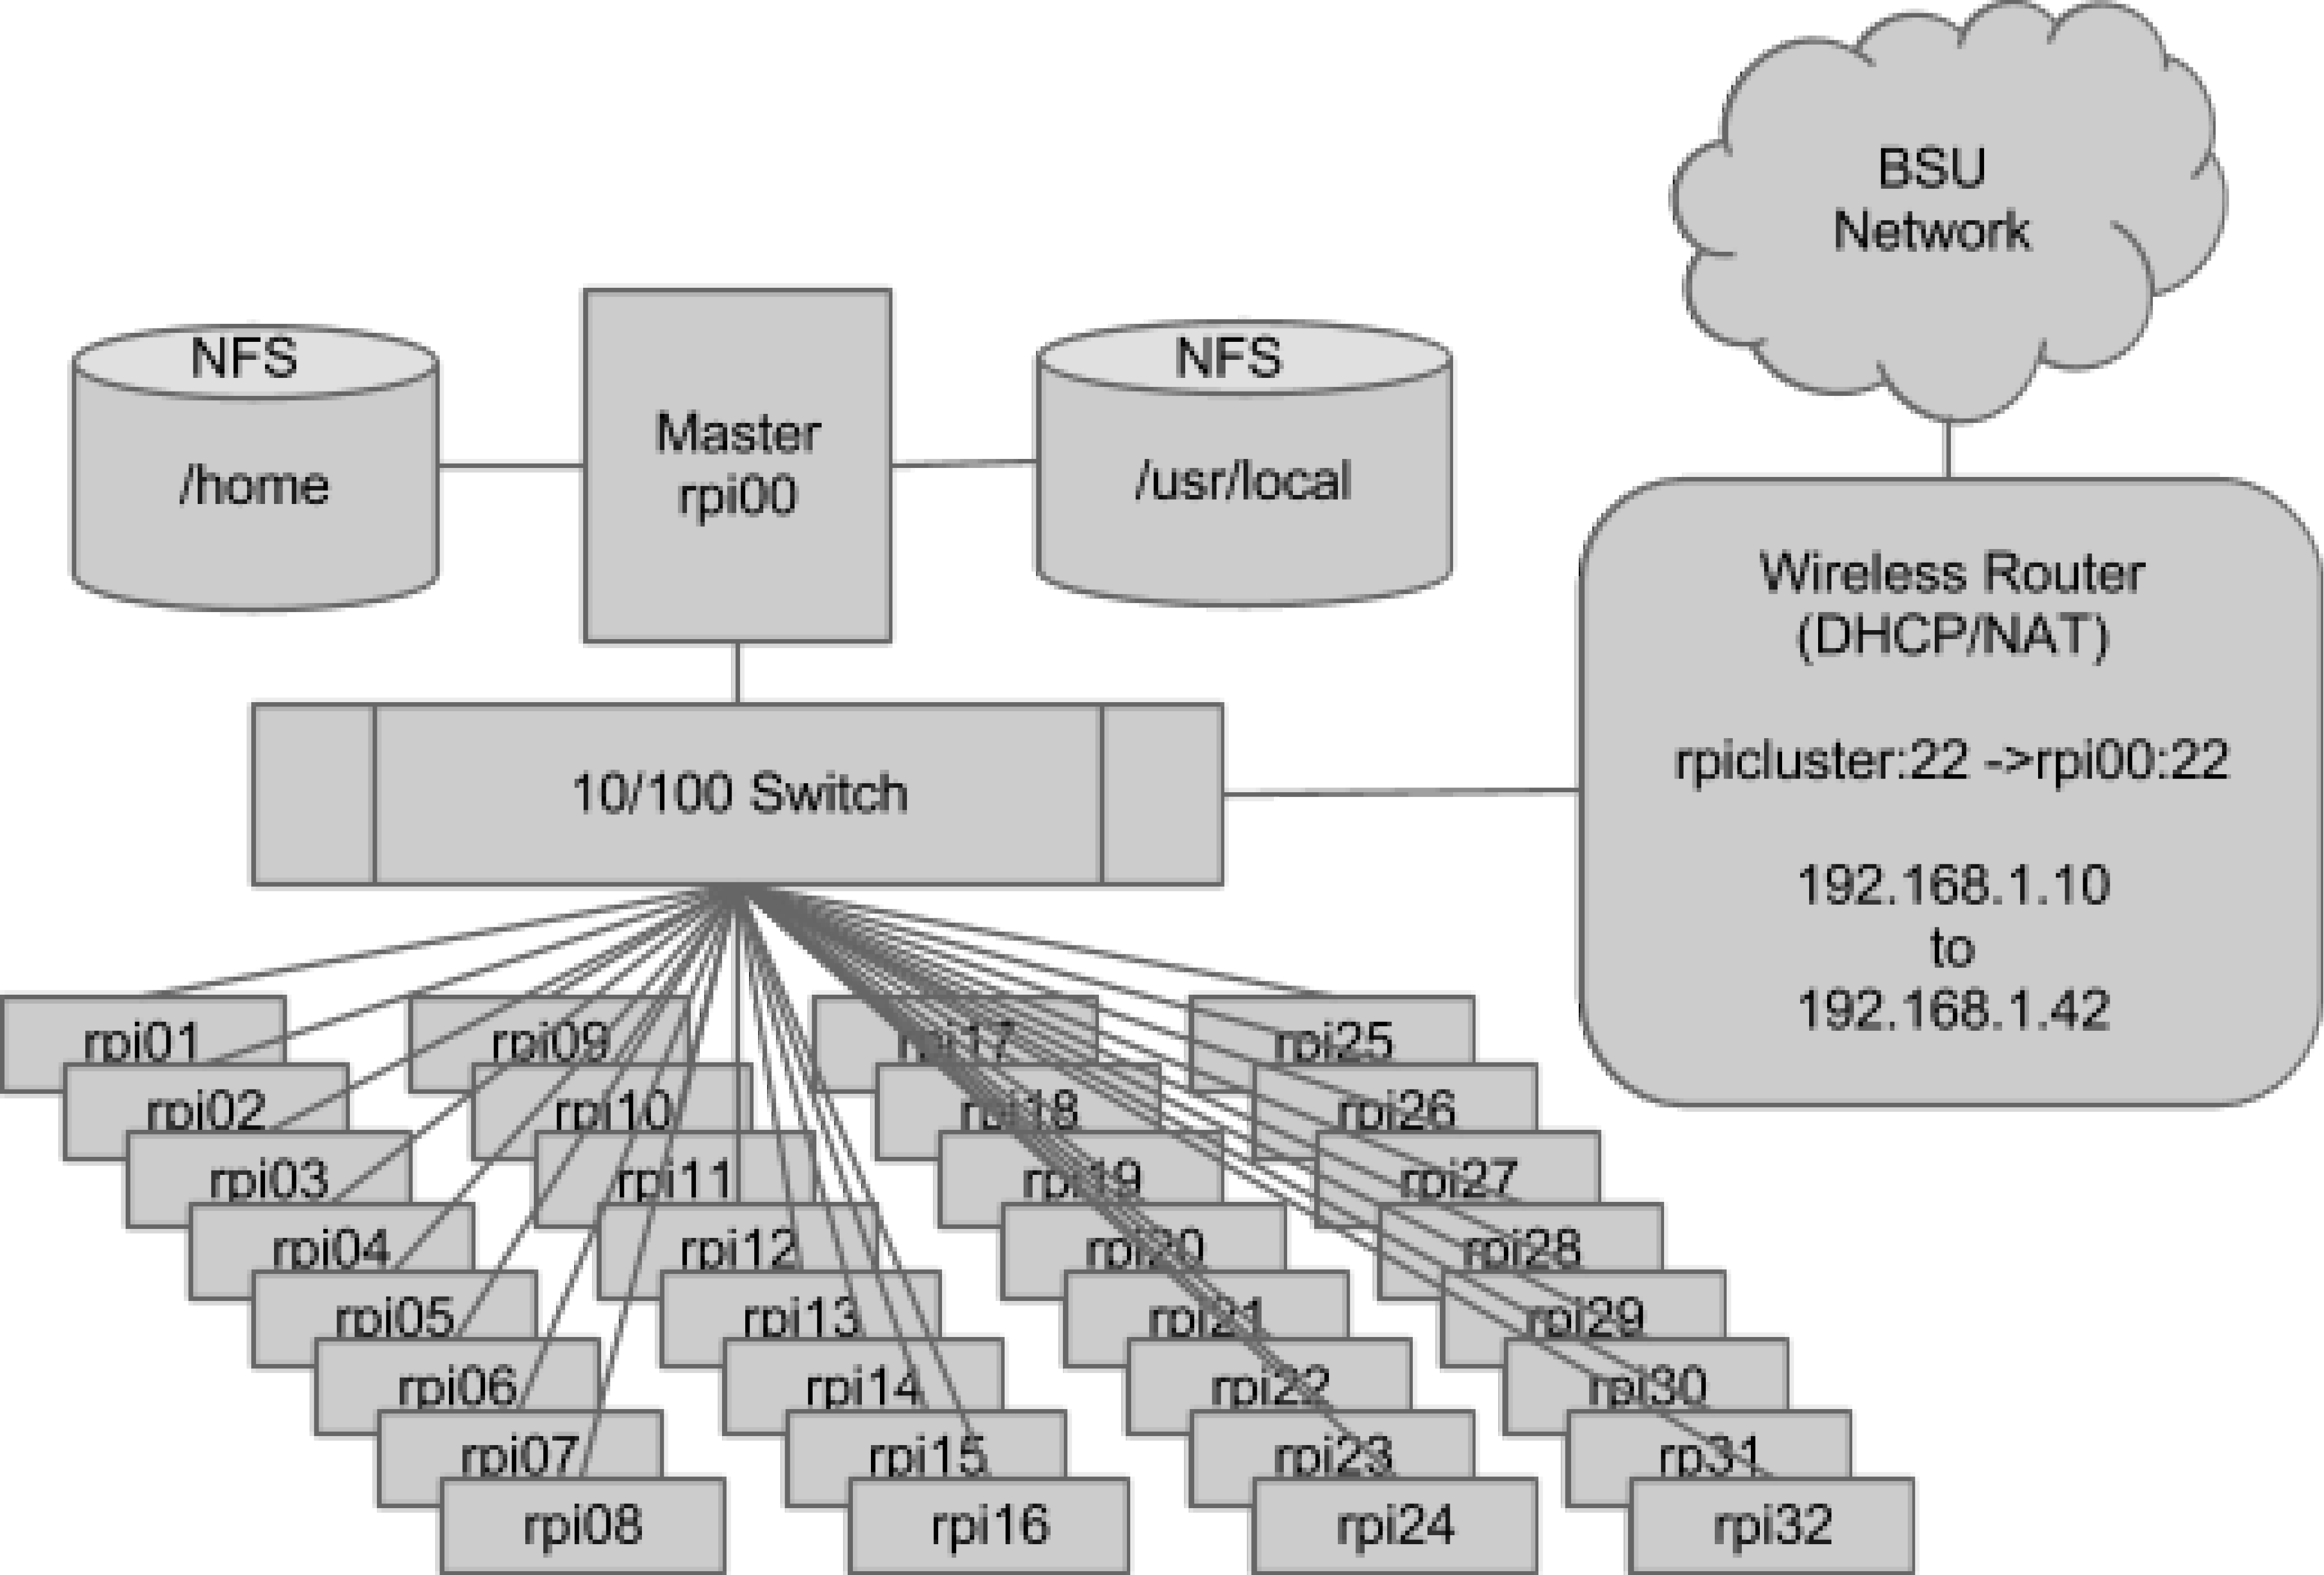
\includegraphics[width=0.4\textwidth]{Chapter4/Figures/kiepert.png}
  \caption[RPiCluster]{Vista general y estructura del sistema (Fuente: Joshua Kiepert)}
  \label{kiepert:structure}
\end{figure}

El coste total del proyecto según Kiepert es de 1967.21 dólares.

\subsubsection{Dramble (Jeff Geerling)}
\label{geerling:dramble}

El clúster \textit{Dramble} está formado por 6 equipos \textbf{Raspberry Pi} capaces de ejecutar en conjunto el gestor de contenidos \textbf{Drupal}\footnote{\href{https://www.drupal.org/}{drupal.org}}. Es utilizado como servidor de pruebas para la ejecución de instancias de este \textit{software} de forma experimental o durante demostraciones en público\cite{geerlingraspberry}. Se compone del conjunto de nodos \textit{Rasbperry Pi} y los mecanismos de red y alimentación que interconectan y proveen de energía a los mismos.

\begin{figure}[H]
  \centering
  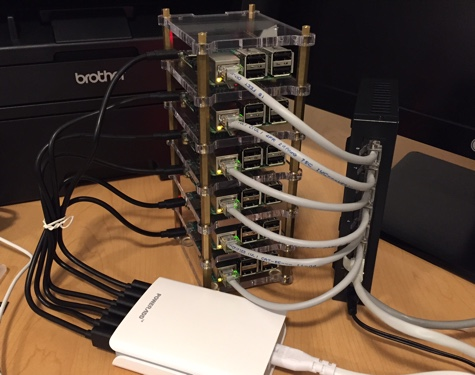
\includegraphics[width=0.4\textwidth]{Chapters/Chapter4/Figures/raspberry-pi-dramble-cluster-wired.jpg}
  \caption[Dramble]{El \textit{Dramble} en ejecución}

\end{figure}
El coste estimado es de 35 dólares por cada Raspberry Pi mas el coste añadido de la red y el cableado de alimentación, totalizando aproximadamente 300 dólares.

\subsubsection{Bramble (GCHQ)}

El organismo gubernamental \textit{Government Communication Headquarters}, agencia de inteligencia del Gobierno Británico, presentó en la \textit{Big Bang Fair} de 2015 un proyecto educativo que combina 66 placas \textit{Raspberry Pi} en un clúster jerárquico con 8 grupos de 8 nodos, cada uno de ellos con un coordinador. El cableado se reduce gracias al uso de la tecnología \textbf{PoE} (\textit{Power over Ethernet}), que provee de conexión a la redes eléctrica y de interconexión a través de un único canal físico. Cada \textbf{Raspberry} cuenta además con un conjunto de elementos adicionales, como un reloj de tiempo real, disco duro externo, cámara, o punto de acceso \textbf{Wi-Fi} \cite{gchqbramble}.

\begin{figure}[H]
  \centering
  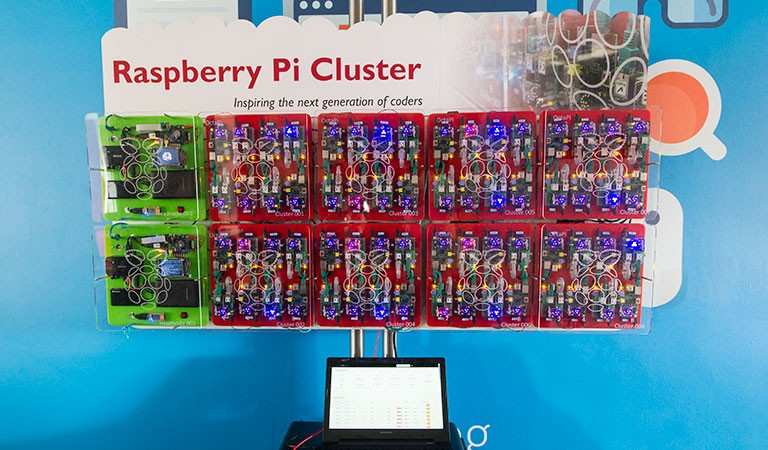
\includegraphics[width=0.8\textwidth]{Chapters/Chapter4/Figures/bramblegchq}
  \caption[Bramble]{Vistazo general de la estructura del sistema Bramble}
  \label{gchq:bramble}
\end{figure}

Se desconocen datos sobre el coste total del sistema.

\subsubsection{Clúster Iridis (Simon Cox, University of Southampton)}

Con el objetivo de atraer a jóvenes estudiantes al mundo de la computación, el profesor Simon Cox crea este clúster con 64 \textbf{Raspberry Pi B} sobre una estructura construida con LEGO\cite{cox:raspberry}. El sistema está diseñado para ejecutar aplicaciones sobre \textit{MPI}. Se desconocen datos sobre el coste total del sistema.

\begin{figure}[H]
  \centering
  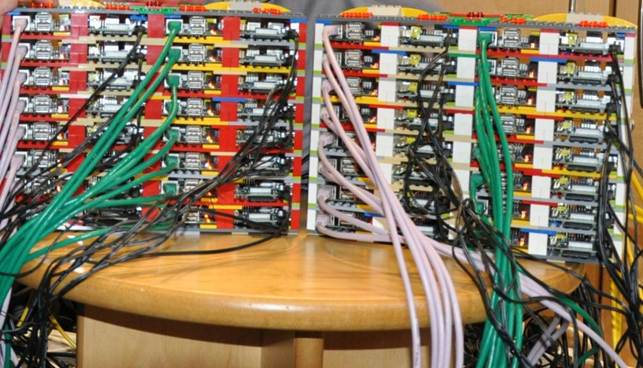
\includegraphics[width=0.65\textwidth]{Chapters/Chapter4/Figures/iridis-pi.jpg}
  \caption[Iridis]{Clúster Iridis}
  \label{cox:iridis}
\end{figure}

\subsubsection{Paralella}

Paralella es un proyecto de la compañía Adapteva que integra en un único chip un conjunto elevado de procesadores independientes con el objetivo de incrementar la capacidad de procesamiento total del sistema a un coste muy reducido, de 99 dólares por unidad \cite{paralella}.

\subsection{Virtualización}

Uno de los mecanismos para crear sistemas distribuidos en auge es la utilización de mecanismos de virtualización (ver \ref{teoria:virtualizacion}, que evitan el uso de diferentes unidades de \textit{hardware}. Estas soluciones se han popularizado en los últimos años principalmente en entornos empresariales, existiendo gran cantidad de proveedores de servicios y herramientas para la creación de un sistema propio (ver \ref{teoria:virtualizacion}). Ejemplos de este tipo de proveedores son \textbf{Amazon Web Services}\footnote{\href{http://aws.amazon.com/}{https://aws.amazon.com}}, \textbf{Google App Engine}\footnote{\href{https://cloud.google.com/appengine/}{https://cloud.google.com/appengine/}}, \textbf{Microsoft Azure}\footnote{\href{http://azure.microsoft.com/}{http://azure.microsoft.com/en-us/}} o \textbf{Digital Ocean}\footnote{\href{http://digitalocean.com}{http://digitalocean.com}}, entre muchos otros. Su éxito reside en su gran versatilidad: es sencillo crear y destruir nuevas réplicas de un sistema bajo demanda, ahorrando costes de forma significativa.

\subsection{\textit{Commercial Off-The-Shelf hardware}}

Este tipo de hardware está constituido por equipos disponibles al público de forma inmediata (\textit{off the shelf}) y generalmente son máquinas de propósito general, las cuales son interconectadas para crear un sistema distribuido que sirva de alternativa a utilidades más potentes, pero de coste superior (como un \textit{mainframe} o un ordenador de mayor potencia). Su coste económico (que se reduce si existe la posibilidad de aprovechar \textit{hardware} existente en la organización, como equipos de escritorio que no están en uso) es su mayor atractivo.

Un ejemplo de este tipo de sistemas son los clústeres \textit{Beowulf}\cite{beowulf:icpp95}, que se construyen sobre una red de área local y un sistema de intercomunicación como \textbf{MPI}, \textbf{PVM} u \textbf{OpenMP}. Existe gran cantidad de documentación para la creación de un clúster de este tipo\footnote{\href{http://tldp.org/HOWTO/Beowulf-HOWTO/}{tldp.org/HOWTO/Beowulf-HOWTO/}}, así como una serie de recursos (sistemas operativos, herramientas\dots) diseñadas con el propósito específico de crear este tipo de sistemas.


\section{Evaluación de alternativas}
\label{alternativas}
A la hora de evaluar las diferentes opciones que satisfagan los requisitos descritos, se consideran los siguientes aspectos:

\begin{itemize}
  \item Coste económico.
  \item Prestaciones técnicas (potencia de procesamiento, entrada/salida, capacidad de almacenamiento,facilidad de interconexión con otros elementos\dots).
  \item Facilidad de trabajo y de aprendizaje (documentación disponible, proyectos similares ya realizados, conocimiento previo sobre la plataforma en cuestión\dots).
  \item Escalabilidad del sistema.
  \item Necesidades de mantenimiento del sistema.
  \item Consumo eléctrico.
  \item Obsolescencia del sistema (periodo de tiempo en el que el \textit{hardware} y \textit{software} del sistema podrán ser actualizados y ser capaces de satisfacer los requisitos para los que fue creado).
\end{itemize}

\begin{table}[H]
\begin{tabular}{|p{2.4cm}|p{12cm}|}
\hline
&\textbf{Virtualización de entornos de trabajo}\\
\hline
Descripción&Crear un conjunto de nodos virtuales dentro de una máquina que simulen un sistema distribuido\\
\hline
Ventajas intrínsecas&Simplificación del sistema (reduce las necesidades de adquisición y mantenimiento de hardware). Gestión de varias partes del sistema (sistema de ficheros centralizado, gestión de usuarios\dots) de forma mas sencilla. El coste se reduce significativamente.\\
\hline
Inconvenientes intrínsecos&No se exploran apenas las posibilidades de un sistema distribuido formado por varios equipos físicamente independientes e impide aprovechar dicha independencia para los objetivos didácticos del sistema.\\
\hline
Facilidad de trabajo&Si bien el trabajo con cada una de las instancias es previsiblemente sencillo, debido a la eliminación de la gran parte del mantenimiento de la capa física subyacente, el uso de este tipo de sistema requiere una etapa de formación previa en materia de virtualización.\\
\hline
Prestaciones técnicas&Las prestaciones técnicas con las que se contaría, de llevarse a cabo este proyecto, son las de los equipos ya dispuestos para fines similares a este en el Centro. Tres equipos Dell PowerEdge r410, con dos procesadores Xeon E5620, 32GB de RAM y disco duro de 500GB en RAID1.\\
\hline
Coste económico&El coste económico es muy reducido si ya se cuenta con los equipos a utilizar y las licencias del \textit{software} de virtualización necesarias.\\
\hline
Escalabilidad&Dependiente de las capacidades de virtualización del equipo disponible, y el número de nodos y usuarios a gestionar.\\
\hline
Mantenimiento&Las necesidades propias de un sistema operativo multiusuario (previsiblemente \textbf{GNU/Linux}) junto a las específicas de la virtualización de los equipos (monitor de máquinas virtuales).\\
\hline
Consumo energético&Se desconocen datos concretos.\\
\hline
Obsolescencia&Se estima una larga vida útil del sistema. Las máquinas virtuales instaladas en un sistema físico son fácilmente trasladables a otro equipo, por lo que la dependencia de la parte física del sistema es muy baja.\\
\hline
Material&Se plantea el aprovechamiento de equipos ya presentes en la infraestructura en la que trabajar, por lo que se estima un coste muy pequeño a la hora de adquirir material.\\
\hline
Análisis coste/beneficio&El coste es muy bajo, dado que no es necesario adquirir ningún equipo. El consumo energético también es bajo, pues estos equipos ya se encuentran en funcionamiento, y añadir un sistema como el que se plantea crear no incrementaría previsiblemente el gasto.\\
\hline
\end{tabular}
\caption[Características de la virtualización de entornos de trabajo]{Evaluación de las características de la virtualización de entornos de trabajo}
\end{table}

\begin{table}[H]
\begin{tabular}{|p{2.4cm}|p{12cm}|}
\hline
&\textbf{Clúster con equipos de escritorio}\\
\hline
Descripción&Crear un conjunto de nodos virtuales dentro de una máquina que simulen un sistema distribuido\\
\hline
Ventajas intrínsecas&La potencia del sistema es mucho mayor que la de cualquier otra solución considerada. Se reduce dramáticamente el coste de adquisición de material y permite dar un nuevo ciclo de vida a material universitario. La arquitectura es conocida y fiable.\\
\hline
Inconvenientes intrínsecos&No se exploran las características únicas de otros sistemas menos ``convencionales'', como los sistemas embebidos. El consumo energético es mayor y existe una mayor demanda de espacio que puede dificultar la implementación de diferentes aplicaciones didácticas ya planteadas como objetivo funcional del sistema.
\\
\hline
Facilidad de trabajo&Soporte completo de casi la totalidad de las distribuciones de GNU/Linux. Las necesidades de manipulación de hardware se minimizan.\\
\hline
Prestaciones técnicas&Los equipos cuentan con una arquitectura x86/x86-64, entre 2 y 4 GB de memoria principal, conectividad Ethernet y USB, así como espacio de almacenamiento en un disco duro. 
%  \vspace{-\topsep}
%  \begin{itemize}[noitemsep]
%   \setlength{\parskip}{0pt}
%   \setlength{\itemsep}{0pt plus 1pt}
%   \item Arquitectura x86/x86-64 (dependiendo de los equipos a utilizar finalmente).
%   \item Entre 2 y 4 GB de memoria principal.
%   \item Conectividad Ethernet, USB.
%   \item Almacenamiento en disco duro.
% \end{itemize}
% \vspace{-\topsep}
\\
\hline
Coste económico&El coste económico de estos equipos es prácticamente nulo, pues ya se cuenta con los mismos y su utilización no exige la adquisición de nuevos equipos que los sustituyan. Estos equipos ya han sido retirados y no están empleados actualmente en ninguna tarea.\\
\hline
Escalabilidad&Dependiente únicamente del coste económico de la adquisición de nuevos equipos, o de la disponibilidad de equipos que no estén utilizados.\\
\hline
Mantenimiento&Las propias de cualquier sistema multiusuario y las específicas del montaje dado (en materia de refrigeración, gestión de cableado, etcétera).
\\
\hline
Consumo energético&El típico de cualquier equipo de escritorio.\\
\hline
Obsolescencia&Estos equipos tienen una antigüedad de aproximadamente 4 años. Dicha edad no impide que sean capaces de utilizar aplicaciones actuales, y en general no se prevé la incompatibilidad con ninguna aplicación. No obstante, son equipos relativamente antiguos que han sido utilizados de forma intensiva, por lo que la probabilidad de fallo en los mismos puede ser elevada.\\
\hline
Material&Se cuenta con un número suficiente de equipos para la creación del sistema final.\\
\hline
Análisis coste/beneficio&Si bien el coste de estos equipos es prácticamente nulo, dicho atractivo contrasta con los potenciales problemas que el uso de estos sistemas puede implicar (obsolescencia, uso de sistemas convencionales en detrimento de soluciones más innovadoras\dots).\\
\hline
\end{tabular}
\caption{Características de un clúster con equipos de escritorio}
\end{table}

\begin{table}[H]
\begin{tabular}{|p{2.4cm}|p{12cm}|}
\hline
&\textbf{Clúster con computadores embebidos}\\
\hline
Descripción&Recientemente han surgido en el mercado sistemas embebidos con capacidad de cómputo elevada y precio muy reducido (en torno a los 40 euros por unidad). Estos equipos destacan además por su versatilidad. La mayoría de ellos son capaces de ejecutar una gran variedad de sistemas operativos (GNU/Linux, RISC OS, BSD, Windows\dots), incluyen una gran cantidad de mecanismos de interconexión y soportan la mayoría de herramientas presentes en equipos de escritorio y servidores.

Se plantea utilizar este tipo de plataformas para la creación del sistema, disponiendo los diferentes equipos en un pequeño ``rack'' con un sistema de alimentación propio centralizado y una conexión directa a la infraestructura local.\\
\hline
Ventajas intrínsecas&Existen varias soluciones similares bien documentadas.
El hardware es flexible, barato y el consumo es pequeño.
Gran comunidad de desarrolladores alrededor de la plataforma.\\
\hline
Inconvenientes intrínsecos&La potencia del sistema es pequeña.\\
\hline
Facilidad de trabajo&Existe una amplia documentación del \textit{hardware} de este tipo de equipos, así como numerosos proyectos basados en los mismos, entre los que se incluyen sistemas similares a la solución planteada. Se cuenta además con experiencia en el manejo de estas placas.\\
\hline
Prestaciones técnicas&Generalmente basados en la arquitectura ARM. Disponen de entre 512 MB y 2GB de memoria principal, conectividad Ethernet, I\textsuperscript{2}C, GPIO y USB. La alimentación se realiza Alimentación a través de un puerto USB o el GPIO.
% \begin{itemize}[noitemsep]
%   \item Generalmente basados en la arquitectura ARM.
%   \item Entre 512 MB y 2 GB de memoria principal.
%   \item Conectividad \textbf{Ethernet},\textbf{I\textsuperscript{2}C}, \textbf{GPIO}, \textbf{USB}.
%   \item Alimentación a través de \textbf{USB}/\textbf{GPIO}.
%   \item Almacenamiento secundario basado en tarjetas microSD/SD, expansible a través de USB.
% \end{itemize}
\\
\hline
Coste económico&Muy reducido, con un coste por nodo de entre 20 y 40 euros, al que se debe añadir los mecanismos de alimentación e interconexión.\\
\hline
Escalabilidad&Dependiente únicamente del coste económico de la adquisición de nuevos equipos.\\
\hline
Mantenimiento&Las mismas que cualquier sistema multiusuario.\\
\hline
Consumo energético&Variable según modelo, entre 3 y 4 W, con 5V de tensión y un amperaje variable entre 0.6 y 0.8 A.\\
\hline
Obsolescencia&El software de terceros (sistema operativo, bibliotecas, etc) a incluir está respaldado por una comunidad extensa que provee actualizaciones de forma continua, por lo que previsiblemente el sistema podrá estar actualizado durante varios años.
Se prevé que las necesidades que el sistema cubre no demandarán una mayor potencia de cálculo en el futuro.\\
\hline
Material&El Departamento de Informática y Automática cuenta con varios de estos equipos actualmente que podrían disponerse para el uso en el proyecto.\\
\hline
Análisis coste/beneficio&\\
\hline
\end{tabular}
\caption{Características de un clúster con computadores embebidos}
\end{table}

\begin{table}[H]
\begin{tabular}{|p{2.4cm}|p{12cm}|}
\hline
&\textbf{Clúster con equipos embebidos multimedia}\\
\hline
Descripción&Utilización de equipos embebidos diseñados para aplicaciones multimedia en el sistema (ejemplos de alternativas comerciales son \textbf{Chromecast}, \textbf{Apple TV}, \textbf{Amazon Fire TV}\dots).\\
\hline
Ventajas intrínsecas&Relación potencia/precio presumiblemente similar o superior a soluciones de coste similar como las placas Raspberry Pi.\\
\hline
Inconvenientes intrínsecos&Dificultad de conexión (generalmente la conexión a red se realiza de forma inalámbrica, ausencia casi absoluta de cualquier conexión cuya finalidad no sea la emisión de contenido multimedia o la conexión con sistemas de almacenamiento), falta de puertos \textbf{GPIO}, \textbf{I\textsuperscript{2}C}\dots\\
\hline
Facilidad de trabajo&Es difícil determinar la viabilidad de esta solución, pues no se cuenta con experiencia previa ni una documentación amplia al respecto. Además, es probable que sea necesaria la manipulación del sistema a muy bajo nivel, lo cual incrementa el grado de complejidad de la solución.\\
\hline
Prestaciones técnicas&Como referencia se utilizan las prestaciones de uno de los equipos más populares, el \textbf{Google Chromecast}\footnote{\href{https://wikidevi.com/wiki/Google\_Chromecast\_\%28H2G2-42\%29}{https://wikidevi.com/wiki/Google\_Chromecast\_\%28H2G2-42\%29}}: Procesador ARM de 2 núcleos a 1.2 GHz. 512 MB de memoria principal. 2 GB de almacenamiento no extensibles. La alimentación se realiza por micro-USB. Utiliza un sistema operativo basado en Google TV, ChromeOS y Android.
% \begin{itemize}[noitemsep]
%   \item Procesador ARM de 2 núcleos a 1.2 GHz.
%   \item 512 MB de memoria principal.
%   \item 2 GB de almacenamiento no extensibles.
%   \item Alimentación por micro-USB.
%   \item Utiliza un sistema operativo basado en \textbf{Google TV}, \textbf{ChromeOS} y \textbf{Android}.
% \end{itemize}
\\
\hline
Coste económico&El coste de estos equipos es reducido, inferior a 30 € por unidad.\\
\hline
Escalabilidad&Dependiente del coste de adquisición de nuevos equipos y las facilidades de interconexión de la plataforma (previsiblemente compleja, debido a la ausencia de otra conexión diferente a la inalámbrica).\\
\hline
Mantenimiento&Dependiente del número de modificaciones que se realicen a las diferentes capas del sistema. En el peor de los casos puede que el administrador tenga que someterse a una etapa de formación para realizar un mantenimiento adecuado del sistema sin depender de los desarrolladores. Otras necesidades son aquellas derivadas del mantenimiento de un sistema multiusuario sumadas a posibles problemas de interconexión si se utiliza una red inalámbrica.\\
\hline
Consumo energético&El diseño de estos equipos está orientado a la minimización del consumo energético, por lo que se estima reducido.\\
\hline
Obsolescencia&La obsolescencia del sistema es difícil de determinar: no se cuenta con una gran cantidad de \textit{software} para este tipo de sistemas más allá de las aplicaciones multimedia. No obstante, el sistema subyacente es conocido (Linux).
Se prevé que las necesidades que el sistema cubre no demandarán una mayor potencia de cálculo en el futuro.\\
\hline
Material&No se dispone de material de estas o similares características.\\
\hline
Análisis coste/beneficio&\\
\hline
\end{tabular}
\caption{Características de un clúster con equipos embebidos multimedia}
\end{table}

\subsection{Elección de la solución}

Basándose en las características descritas anteriormente, se elige realizar el sistema utilizando sistemas embebidos de bajo coste en virtud de los siguientes aspectos positivos.

\begin{itemize}[noitemsep]
\item Compatibilidad con de gran cantidad de \textit{software} y sistemas operativos.
\item Versatilidad y facilidad de interconexión.
\item Se cuenta con experiencia en el uso de este tipo de dispositivos.
\item Bajo coste.
\end{itemize}

Dentro de las diferentes alternativas, se escoge la placa \textbf{Raspberry Pi} como modelo concreto.

%\end{comment}
\subsection{Raspberry Pi: Elección de las características básicas del sistema}

Se opta por las placas de la familia \textbf{Raspberry Pi} para la realización el sistema debido a la gran cantidad de soporte con el que cuentan, tanto por parte de la fundación \textbf{Raspberry Pi} como por diferentes comunidades de desarrolladores. Es el computador de este tipo que más sistemas operativos soporta\footnote{\href{http://elinux.org/RPi_Distributions}{http://elinux.org/RPi\_Distributions}} y existen gran cantidad de proyectos que dotan de mayor funcionalidad al sistema y que generalmente son diseñados para aprovechar las características del \textit{hardware} específico de la máquina.


\begin{landscape}
\begin{table}[h]
\begin{tabular}{|p{3.2cm}|p{6cm}|p{6cm}|p{6cm}|}
\hline
 & \textbf{Modelo B} & \textbf{Modelo B+} & \textbf{Modelo B 2}\\ \hline
\textbf{Procesador} & ARMv6 1 Núcleo, 700 MHz (safe overclock hasta 1GHz) & ARMv6 1 Núcleo, 700 MHz (safe overclock hasta 1GHz) & ARMv7 4 Núcleos a 900 MHz\footnote{\href{https://learn.adafruit.com/embedded-linux-board-comparison/performance}{https://learn.adafruit.com/embedded-linux-board-comparison/performance} En este artículo se realiza un análisis sobre el rendimiento de diferentes placas de este tipo}\footnote{\href{https://learn.adafruit.com/introducing-the-raspberry-pi-2-model-b/performance-improvements}{https://learn.adafruit.com/introducing-the-raspberry-pi-2-model-b/performance-improvements} Artículo sobre las mejoras de rendimiento de la Raspberry Pi 2 frente a los modelos originales} \\ \hline
\textbf{Memoria} & 512 MB compartidos con GPU & 512 MB compartidos con GPU & 1 GB compartido con GPU\\ \hline
\textbf{LINPACK} \cite{hackaday:benchmarkpi2,gist:linpackbenchmark,elinux:benchmark} & 40.64 & 40.64 & 92.88\\ \hline
\textbf{Conexiones} & 2 USB, GPIO de 8 pines. Ethernet 10/100 & 4 USB, GPIO de 17 pines. Ethernet 10/100 & 4 USB, GPIO de 17 pines. Ethernet 10/100\\ \hline
\textbf{Consumo medio} & 700 mA, 5 V (3.5 W) & 600 mA, 5 V (3 W) & 800 mA, 5 V (4 W)\footnote{\href{http://raspi.tv/2014/how-much-less-power-does-the-raspberry-pi-b-use-than-the-old-model-b}{http://raspi.tv/2014/how-much-less-power-does-the-raspberry-pi-b-use-than-the-old-model-b} Mejoras de consumo en el modelo 2.}\\ \hline
\textbf{Almacenamiento} & SD & microSD & microSD\\ \hline
\textbf{Alimentación} & Mediante micro-USB o los pines GPIO & Mediante micro-USB o los pines GPIO &Mediante micro-USB o los pines GPIO\\ \hline
\textbf{Sistemas operativos compatibles} & 

Arch Linux ARM, OpenELEC, Puppy Linux, Raspbmc, RISC OS, Raspbian, XBian, openSUSE, Slackware ARM, FreeBSD, Plan 9, Kali Linux, Sailfish OS, Pidora (Fedora Remix), Lista completa en \footnote{\href{http://elinux.org/RPi\_Distributions}{http://elinux.org/RPi\_Distributions}} & Los mismos que para el modelo B & Hasta la fecha, únicamente:

Ubuntu Snappy Core, Raspbian, OpenELEC, RISC OS, Según la web de Arch Linux, también soporta este sistema operativo \footnote{\href{http://archlinuxarm.org/platforms/armv7/broadcom/raspberry-pi-2}{archlinuxarm.org/platforms/armv7/broadcom/raspberry-pi-2}} \\

\hline % 

\textbf{Otros} & Modelo descatalogado, el soporte oficial y proporcionado por la comunidad probablemente será menor que para los modelos más recientes en el futuro. &  & Lleva poco tiempo en el mercado (apenas un mes). Se conocen pequeños fallos en el hardware (fotosensibilidad de algún componente).\\ \hline

\end{tabular}
\caption[Comparativa de las características relevantes de los diferentes modelos de Raspberry Pi]{Comparativa de las características relevantes de los diferentes modelos de Raspberry Pi.
Quedan descartados los modelos A y A+ por la carencia de puerto Ethernet (además de otras características necesarias).}
\end{table}
\end{landscape}

\begin{landscape}
\subsection{Elección del sistema operativo}
\label{os:evaluation}
\begin{table}[h]
\begin{tabular}{|p{1.7cm}|p{4.7cm}|p{4.7cm}|p{3cm}|p{5cm}|p{2cm}|}
\hline
\textbf{Nombre} & \textbf{Enfoque} & \textbf{Características notables} & \textbf{Ventajas} & \textbf{Inconvenientes} & \textbf{Software disponible}\\ \hline
\textbf{Arch Linux ARM} & Distribución ligera centrada en el minimalismo y la disponibilidad de software novedoso. Requiere que el usuario esté familiarizado con GNU/Linux. & Muy optimizado con un ciclo de desarrollo que permite contar con software puntero en poco tiempo. & Eficiente, gran comunidad alrededor, relativamente sencillo de utilizar. & En ocasiones puede ser complejo su uso. Ya no se incluye en las distribuciones por defecto de la Fundación Raspberry Pi, lo cual puede suponer falta de soporte oficial. & 8700 y 57000 en el \textbf{AUR}\footnote{\textit{Arch User Repository}: \href{https://aur.archlinux.org/}{https://aur.archlinux.org/}}\\ \hline

% 8700 paquetes disponibles en los repositorios oficiales  ()\\ \hline

\textbf{Ubuntu Snappy Core} & Centrado en la facilidad de uso. & Es la distribución más popular (en equipos de escritorio) contando con gran cantidad de \textit{software} disponible & Fácil de configurar, gran cantidad de soporte & Recientemente portado a la Raspberry de forma intensiva.El rendimiento de Ubuntu suele ser menor al de otros sistemas operativos debido a la gran cantidad de paquetes incluidos por defecto. & Unos 40000\footnote{\href{https://launchpad.net/ubuntu/trusty/armhf}{https://launchpad.net/ubuntu/trusty/armhf}}\\ \hline 

\textbf{Raspbian} & Centrado en la estabilidad del sistema en detrimento de las últimas versiones de los componentes del sistema. & Es el sistema más utilizado en la plataforma Raspberry Pi. La fundación Raspberry Pi promociona su uso y la mayoría de los desarrolladores crean herramientas para este sistema. & Estable, gran cantidad de \textit{software} disponible, ya conocido. & La instalación básica del sistema incluye una gran cantidad de herramientas que consumen recursos del sistema de forma significativa. & Unos 20000\\ \hline
\end{tabular}
\caption{Comparativa de sistemas operativos (1)}
\end{table}
\end{landscape}

\begin{landscape}
\begin{table}[h]
%\begin{tabular}{|p{2cm}|p{4cm}|p{5cm}|p{3cm}|p{4cm}|p{3.5cm}|}
\begin{tabular}{|p{1.7cm}|p{4.7cm}|p{4.7cm}|p{3cm}|p{5cm}|p{2cm}|}
\hline
\textbf{Nombre} & \textbf{Enfoque} & \textbf{Características notables} & \textbf{Ventajas} & \textbf{Inconvenientes} & \textbf{Software disponible}\\ \hline

\textbf{RISC OS} & Diseñado específicamente para la arquitectura ARM, aprovechando las posibilidades de dicha arquitectura al máximo. & Eficiente, basado en el RISC OS original, incluyendo características del mismo. Sistema monousuario con multitarea cooperativa (en contraste con multihilo o multitarea apropiativa). & Muy eficiente & No esta basado en un sistema conocido previamente. Relativamente desfasado en cuanto a la arquitectura del sistema operativo. El software suele ser programado en BBC BASIC (con el que no se cuenta experiencia). & No se conocen cifras\\ \hline

\textbf{Gentoo} & Diseñado para permitir la modificación del sistema al máximo nivel posible. Todo el \textit{software} es compilado en la máquina que lo instala, en lugar de utilizar ejecutables precompilados & Enfocado en maximizar el grado de personalización del sistema. & Permite ser modificado de forma sencilla. & Poco soportado en Raspberry Pi. & No se conocen cifras\\ \hline

\textbf{Windows 10} & Diseñado para el paradigma del Internet de las Cosas, & Sencillo de utilizar, con soporte (previsiblemente) del \textit{framework} \textbf{.NET}. & Soporta un conjunto de tecnologías ya conocidas pero no compatibles con otras alternativas. El soporte de \textbf{.NET} constituiría una ventaja clave.& Aún no se encuentra disponible\cite{windows10raspberry}. Esta diseñado para un propósito especifico. No compatible con software para Linux de forma nativa. & No se conocen cifras\\ \hline

\end{tabular}
\caption{Comparativa de sistemas operativos (2)}
\end{table}
\end{landscape}


\section{Ingeniería de sistemas: propuesta de solución definitiva}

En esta sección se describen los aspectos a alto nivel sobre todos los componentes que se integrarán en el sistema final (tanto \textit{hardware} como \textit{software}), así como las relaciones entre los mismos. En función de la evaluación llevada a cabo se extraen las siguientes decisiones de diseño que conforman la propuesta de solución definitiva.

\subsection{\textit{Hardware}}

\subsubsection{Nodos}

Todo el sistema se construirá sobre placas \textbf{Raspberry Pi 2} debido a su alta versatilidad, gran potencia de cálculo, interfaces de comunicación, soporte por parte de las diferentes comunidades de desarrolladores, coste y bajo consumo eléctrico.

\subsubsection{Equipos auxiliares}

En caso de que sea necesario integrar algún nodo en el sistema se utilizarán equipos \textbf{COTS} en desuso presentes en la infraestructura. La utilización de este tipo de nodos se realizará siempre con carácter auxiliar (p.ej. para ofrecer un servicio que sea difícil de soportar por los nodos principales).

\subsubsection{Interconexión física}

El sistema deberá interconectar los diferentes nodos utilizando la red presente en la organización. No obstante se plantea el uso de dispositivos de enrutado o conmutación para mejorar del rendimiento.

\subsubsection{Alimentación}

La alimentación del sistema deberá proceder de una única fuente, a fin de minimizar las cantidades de  cableado, transformadores u otro tipo de elementos.

\subsubsection{Estructura}

Se deberá diseñar una estructura propia que recoja todos los componentes del sistema, a fin de facilitar la instalación en su ubicación final.

\subsection{\textit{Software}}

\subsubsection{Sistema operativo}
\label{problema:sistemaoperativo}

El sistema operativo a utilizar será \textbf{Arch Linux ARM}, debido a la gran comunidad de soporte con la que cuenta, compatibilidad con la gran mayoría de componentes presentes en un sistema GNU/Linux y modelo arquitectónico que apuesta por la simplicidad, ``limpieza'' y eficiencia del sistema.

Se partirá de la instalación base del sistema operativo debido a que incluye el conjunto más pequeño de herramientas con el que el sistema operativo es capaz de trabajar, añadiendo posteriormente aquellos paquetes necesarios para la construcción del sistema. Este enfoque evita la inclusión de \textit{software} innecesario que afectaría negativamente al rendimiento de la solución final.

\subsubsection{Componentes del sistema operativo}

Se crearán un conjunto de componentes que se integrarán en el sistema operativo y podrán ser aprovechados por aplicaciones creadas por usuarios o por herramientas internas del propio sistema. Dichos servicios incluyen mecanismos de descubrimiento, coordinación, acuerdo, autoconfiguración de componentes o gestión de usuarios, entre otros.

\subsubsection{Interfaces de conexión entre componentes}

Aquellos servicios ofrecidos por el sistema operativo que sean aprovechables por los usuarios finales deberán ofrecer una interfaz de conexión con los mismos. Dicha interfaz deberá apoyarse en mecanismos de interconexión conocidos y deberá ofrecerse en el mayor número de plataformas y lenguajes de programación posible.

\subsubsection{Servicios}

El sistema se plantea como un conjunto de nodos que ofertan servicios consumibles por otros componentes o terceras partes. Dichos servicios deberán contar con una serie de puntos de acceso claramente definidos que constituirán las interfaces de uso de dichos servicios.

\subsubsection{Instalación y mantenimiento}

El sistema final se compondrá de un conjunto elevado de nodos, por lo que se espera que la instalación y configuración de los mismos sea un proceso tedioso. A fin de minimizar dicha carga de trabajo se crearán herramientas que automaticen dichas etapas, idealmente, de forma completa.

\subsubsection{Herramientas de desarrollo a utilizar}

Se plantea el uso del lenguaje de programación Python\footnote{\href{http://www.python.org}{http://python.org}} como herramienta principal de desarrollo, debido a su potencia de cálculo y simplicidad, que permite crear aplicaciones demandantes de pocos recursos (aspecto vital, máxime cuando se utilizará sobre un sistema con un \textit{hardware} poco potente) de forma sencilla y rápida. También se plantea el uso de los lenguajes de programación C y C++ para el desarrollo de herramientas a bajo nivel, así como herramientas web para el desarrollo de aplicaciones utilizadas por el usuario.

\section{Integración}

El sistema se integrará en la organización objetivo utilizando diferentes recursos de la misma, como la red que interconecta todos los equipos o el mecanismo de autenticación.

\section{Proceso}

La determinación del proceso de desarrollo del sistema influirá significativamente en la consecución de los diferentes objetivos marcados.

Las particulares características cada proyecto propician la elección de un proceso u otro. En el caso concreto del proyecto en cuestión se deben considerar las siguientes características:

\begin{itemize}

\item No se cuenta con experiencia previa en la construcción de varios componentes cruciales. Serán necesarias etapas de aprendizaje y la tolerancia a decisiones erróneas deberá ser alta.

\item El proyecto tiene un alto componente de experimentalidad: el sistema final será el resultado de los diferentes procesos de investigación y prueba de soluciones para cada uno de los problemas planteados. La incertidumbre es por tanto alta, y por ello la toma de decisiones debe ser reversible, a fin de poder cambiar el enfoque aplicado a un problema si se detecta que los resultados del mismo serán infructuosos. Dicha reversibilidad implica principalmente la capacidad de poder rectificar en un periodo de tiempo pequeño, debido principalmente a la restricción de tiempo que el proyecto incluye.

\item Es esperable que los requisitos definidos en las diferentes fases del proyecto deban ser modificados debido a la gran incertidumbre con la que se debe lidiar.

\end{itemize}

Es por todo ello que es necesaria la determinación de un proceso de desarrollo que deje espacio a etapas de aprendizaje y experimentación, así como la modificación de los diferentes requisitos preestablecidos. 

\subsection{Elección del proceso}
\label{process}
En virtud de las razones expuestas se opta por un proceso ágil apoyado sobre prototipos. 

Un prototipo es un componente \textit{software} que implementa un subconjunto de la funcionalidad del sistema final y es operativo. El desarrollo de prototipos permite realizar evaluaciones de la funcionalidad implementada de forma efectiva ahorrando costes y tiempo de desarrollo. En el caso concreto de este proyecto posibilitan la evaluación de una alternativa sobre el resto, así como la viabilidad de una solución sobre el resto. Se apuesta por un modelo de desarrollo de prototipos evolutivo\cite{10.1109/TSE.1975.6312870}, creando versiones funcionales que paulatinamente crezcan en complejidad. Este tipo de prototipado permite experimentar con una estrategia de desarrollo (probar un algoritmo, experimentar con un lenguaje de programación, aprovechar una biblioteca, \textit{framework}\dots) y analizar las ventajas e inconvenientes de la misma en poco tiempo, siendo posible desechar el prototipo en caso de que el camino elegido no satisfaga los requisitos planteados.

Los procesos ágiles suelen ser utilizados a la hora de realizar un proyecto en equipos pequeños en entornos cambiantes o con un grado de incertidumbre muy alto. Procesos ``tradicionales'', como el desarrollo \textit{en cascada} o el lineal no responden de forma dinámica a dichas propiedades, y su adaptabilidad es menor.

En el caso del presente proyecto, se opta por un proceso ágil basado en iteraciones de corta duración (entre 7 y 12 días) con una serie de objetivos definidos y producen una versión más avanzada de los prototipos. Debido a que el proyecto comprende el desarrollo de una serie de productos independientes que conforman un sistema (en contraste con un único producto monolítico final) es necesario paralelizar el desarrollo de todos los procesos a lo largo de las diferentes iteraciones, balanceando la carga de trabajo entre las diferentes tareas.

\subsection{Desarrollo de subsistemas}
Los diferentes aspectos relativos al desarrollo de cada uno de los subsistemas se definen en los anexos dispuestos a tal efecto.

\subsection{Integración del sistema}

Se ha realizado un proceso de integración creciente de los diferentes prototipos creados como resultado de cada uno de los ciclos de desarrollo. Esta práctica es de utilidad para detectar diferentes fallos en el sistema o anomalías fruto de las interacciones entre componentes de forma temprana.

\subsection{Instalación del sistema}

Se han creado herramientas que facilitan la instalación del sistema (ver \ref{marcobootstrap}) en diferentes tipos de infraestructuras que cuenten con una serie de propiedades mínimas (que se reducen a una conexión de red funcional).

\subsection{Evolución del sistema}

La solución presentada es altamente escalable y existe un equipo de soporte para todos los componentes el \textit{software} utilizado, aspectos que garantizan la inclusión de nuevas características y el mantenimiento de los paquetes instalados.  

\subsection{Desmantelamiento del sistema}

Ningún componente contiene materiales cuya manipulación incorrecta pueda dañar su entorno. En el caso de que el desmantelamiento no se produzca por fallos en el \textit{hardware} del sistema, sus componentes pueden ser aprovechados para otros proyectos académicos o profesionales por su poseedor. Los diferentes paquetes \textit{software} no dependen del hardware del sistema para funcionar, salvo varias excepciones, tales como herramientas creadas para un problema concreto de esta plataforma\footnote{Como Marcobootstrap, entre otros}.

%TODO: IS 1 T2 Pg 34
Fases
\begin{itemize}
  \item Definición de requisitos
  \item Diseño
\end{itemize}

\subsection{Planificación temporal}


La planificación temporal del proyecto se realiza en base a las diferentes iteraciones llevadas a cabo. Al finalizar una de las fases, se realiza una reunión con todo el equipo de desarrollo y se analiza el estado de las nuevas versiones de los prototipos, problemas que se han dado y nuevas vías de actuación. A partir de este análisis se determinan los objetivos a cumplir en la siguiente iteración.

Toda la planificación temporal del proyecto se encuentra en el anexo \citationneeded[TODO].

\chapter{Análisis y diseño}
\lhead{Análisis y diseño}
\label{chapter:analisis}

\begin{cabstract}
En el que se describen los diferentes aspectos de las fases de análisis y diseño del sistema desde una perspectiva holística.
\end{cabstract}

\section{Análisis}

Recoger todos los aspectos de análisis de un sistema como el creado en un único capítulo es contraproducente para la adecuada comprensión de los diferentes procesos llevados a cabo. Es por ello que en el presente capítulo se detallarán los diferentes aspectos de análisis para el sistema como unidad, que ayudarán a la identificación de las necesidades a satisfacer por el mismo. Dichos aspectos serán de utilidad durante el desarrollo de las restantes etapas de análisis centradas en cada uno de los diferentes componentes del sistema.

\subsection{Identificación de componentes}

Todo sistema se compone del conjunto de integrantes y las relaciones que estos mantienen entre ellos mismos y su entorno, con una serie de objetivos a cumplir a través de dichas interacciones. El límite entre el sistema y su entorno es de necesario estudio para comprender los diferentes procesos de  entrada y salida que se desarrollan.

\subsubsection{Componentes principales} 

Los componente principales del sistema son los nodos Raspberry Pi, que serán los encargados de la ejecución de las diferentes tareas solicitadas por los usuarios del sistema.

\subsubsection{Componentes secundarios}

En una primera instancia del proceso de análisis no se detalla ningún tipo de nodo secundario, delegando en los componentes principales del sistema todas las tareas a llevar a cabo.

Sin embargo, en las diferentes etapas de desarrollo se plantea el uso de varios componentes secundarios para la gestión de una serie de tareas cuya ejecución en el conjunto de componentes principales es dificultosa, o su delegación beneficia al conjunto de nodos principales. En cualquier caso, dichas tareas pueden ser asignadas a los componentes principales en cualquier momento (ver \ref{chapter:serviciosauxiliares}).

\begin{figure}[H]
  \centering
  \includegraphics[width=0.8\textwidth]{Chapter4/Figures/Análisis-Componentes}
  \caption[Análisis de componentes]{Análisis de componentes del sistema}
  \label{analisis:componentes}
\end{figure}

\subsubsection{Interconexión}

Se plantea el uso de cableado físico Ethernet para la comunicación entre los diferentes nodos. Este tipo de conexión es soportada por todos los componentes anteriormente mencionados, y se cuenta con dicho cableado en la infraestructura del centro (ver \ref{dominioproblema:infraestructura}).

\subsection{Información gestionada por el sistema}

Se plantea un conjunto de requisitos de información gestionados por el sistema pequeño, sin embargo de alta sensibilidad, que el siguiente conjunto de datos.

\subsubsection{Credenciales de usuario}

Claves de acceso al sistema. Generalmente estas se componen de un par usuario-contraseña. Sin embargo, también se contemplan sistemas alternativos, como la autenticación de en clave pública. La manipulación de la identidad del usuario también es un aspecto clave del sistema.

\subsubsection{Archivos personales}

Junto a las claves de usuario es necesario gestionar los diferentes ficheros de trabajo que los usuarios manipulen y almacenen en el sistema. Esto implica proporcionar los diferentes mecanismos de acceso a dichos datos y un mecanismo de privilegios (lectura, escritura, ejecución) para impedir la manipulación de forma no deseada de los mismos.

\subsubsection{Ficheros de configuración e información del sistema}

Diversos componentes del sistema utilizan mecanismos de cifrado cuyas claves no deben ser conocidas por ninguna entidad mas que el administrador del sistema. Los ficheros de configuración del sistema y de las diversas aplicaciones a construir no deben ser modificables por usuarios no autorizados, pues definen aspectos del comportamiento del sistema que pueden comprometer la integridad del mismo si son modificados con fines perniciosos.

\subsubsection{Registros}

Diversos registros del comportamiento del sistema y de las operaciones realizadas en el mismo serán almacenados en el sistema para su posterior análisis. Dichos ficheros pueden incluir información sensible, como datos de usuarios, por lo que el acceso a los mismos deberá estar restringido.

\subsubsection{Información de estado}

Si bien la mayor parte de la información se describe en ficheros de carácter permanente, una parte de la información de importancia en el sistema es generada y gestionada por las propias aplicaciones sin almacenar la misma en ningún tipo de soporte permanente. La volatilidad de la información hace que la versatilidad de la misma sea mayor, sin embargo, será necesario contar con una serie de mecanismos que preserven la información frente a circunstancias como recargas de información, reinicios. La manipulación de este tipo de información (actualizaciones, consulta, modificación) presenta una serie de aspectos diferentes a los propios de las estructuras de datos tradicionales.

\subsubsection{Equipo de soporte}

Como equipos de soporte se plantea el uso del almacenamiento presente en los nodos principales, utilizando, en caso de que sea conveniente, algún nodo secundario como almacén de información.

\section{Identificación de transacciones}

Se plantean los siguientes tipos de transacciones. La frecuencia estimada de estas operaciones se debe determinar en fases posteriores basados en las estadísticas del sistema actual (ver \ref{dominio:estadisticas}).

\begin{itemize}
  \item Operaciones de usuario
    \subitem Autenticación contra el sistema.
    \subitem Ejecución y diseño de trabajos a realizar por el sistema.
    \subitem Realización de pruebas de algoritmos y despliegues.
    \subitem Almacenamiento de ficheros.
  \item Operaciones de administración.
    \subitem Actualizaciones del sistema.
    \subitem Operaciones rutinarias de mantenimiento.
    \subitem Acceso y análisis de registros.
\end{itemize}

\subsection{Evolución del sistema}

En caso de proporcionar una solución exitosa para el conjunto de problemas a resolver por el sistema, es esperable un incremento en el número de componentes principales con el fin de aumentar su capacidad de cómputo. Por ello, la escalabilidad del sistema debe ser uno de los requisitos fundamentales del mismo.

% \subsection{Adquisición del sistema}

% Los aspectos de la adquisición de los diferentes componentes se definen en \ref{adquisicion}

\subsection{Identificación de usuarios}

Los siguientes usuarios harán uso del sistema de forma directa o indirecta\footnote{En los diferentes documentos de análisis adjuntos se detalla la interacción de cada entidad con cada uno de los componentes del sistema de forma más detallada, sirviendo esta enumeración como vista global de los diferentes agentes.}.

\subsubsection{Desarrolladores}

Son aquellos individuos que utilizan el sistema como herramienta de creación y prueba de aplicaciones distribuidas.

\subsubsection{Estudiantes}

Utilizan la plataforma como herramienta para la elaboración de trabajos académicos relacionados con el área de conocimiento de la computación distribuida y como mecanismo para facilitar el estudio de dicha rama.

\subsubsection{Profesorado}

Docentes de las áreas anteriormente mencionadas, que utilizarán el sistema para planificar diferentes ejercicios didácticos a resolver por los alumnos.

\subsubsection{Administradores}

Realizan tareas de mantenimiento en el sistema.

\section{Diseño}

\subsection{Ámbito del sistema}

Se distinguen dos tipos de nodos en el sistema. Los nodos principales se agruparán en una misma ubicación física y llevarán a cabo todas las tareas principales del sistema. De forma complementaria y accesoria existirán nodos especializados en una tarea que se les delegará. Las características de estos nodos (tiempo de computación superior, información almacenada en ellos\dots) hacen que el rendimiento del sistema aumente gracias al proceso de delegación.

\subsection{Diseño de datos}

Se plantean de forma global las siguientes fuentes de datos.

\subsubsection{Estructuras de archivo}

\begin{itemize}
  \item Directorio LDAP.
  \item Bases de datos.
  \item Directorios de usuario.
  \item Ficheros de configuración.
  \item Ficheros de \textit{log} para registrar todas las operaciones llevadas a cabo por el sistema, situaciones irregulares\dots, con el objetivo de ser analizados posteriormente.
\end{itemize}

\subsection{Diseño arquitectónico}

Se plantea el siguiente esquema arquitectónico:

\begin{itemize}
\item Un conjunto de nodos principales centralizados en una misma localización física.
\item Varios nodos secundarios a los que se delegará una serie de tareas. Sus características (mayor capacidad de procesamiento, \textit{hardware} exclusivo\dots hacen que esta delegación mejore el rendimiento global del sistema o cualquier otra propiedad).
\item Mecanismos de interconexión, enrutado y alimentación.
\end{itemize}

\subsection{Diseño de la interfaz}

Las interfaces de acceso al sistema son las siguientes:

\begin{itemize}
\item Acceso mediante SSH
\item Interfaces web, descritas en la documentación adjunta referente a cada una de las herramientas creadas o utilizadas.
\end{itemize}
\subsection{Diseño procedimental}

Todos los aspectos de programación (algoritmos empleados, ejemplos de código) se reflejan en la documentación adjunta referente a cada una de las herramientas creadas o utilizadas.

\subsection{Pruebas}

Se ha utilizado un desarrollo dirigido por pruebas en la mayoría de las herramientas creadas, como se detalla en la documentación técnica que acompaña a cada una de ellas, así como una batería de pruebas de una de las últimas versiones del sistema, como se detalla en \citationneeded[TODO].

\subsection{Entorno tecnológico del sistema}

El sistema se integrará en la Facultad de Ciencias de la Universidad de Salamanca. Todos los aspectos de esta organización se definen en \ref{dominioproblema:infraestructura}.

\subsection{Plan de desarrollo e implementación}

El plan de desarrollo del sistema plantea las siguientes fases:

\begin{itemize}
\item \textbf{Febrero de 2015 a Julio de 2015}: Desarrollo de todo el sistema (\textit{hardware}, \textit{software}, pruebas de integración e instalación.)
\item \textbf{Principios de septiembre de 2015}: Etapa de formación a los diferentes usuarios (profesores, administradores), y primeras pruebas masivas.
\item \textbf{Septiembre de 2015-Junio de 2015}: Integración no definitiva del sistema en diferentes asignaturas.
\item \textbf{Junio de 2015 en adelante}: Integración definitiva del sistema.
\end{itemize}

%\subsection{Adquisición}

\subsection{Adquisición del sistema}
\label{adquisicion}
Antes de realizar cualquier operación de adquisición de componentes es necesario analizar diferentes factores, como las diferentes alternativas viables o soluciones de coste menor o incluso nulo.

En el caso del presente proyecto, la adquisición de una serie de componentes no es opcional, pues no se cuenta con ellos previamente. Tras evaluar diferentes opciones, se decide adquirir los siguientes componentes:

\begin{itemize}
  \item Nodos \textbf{Raspberry Pi}.
  \item Cables de alimentación.
  \item Tarjetas SD/micro-SD (soporte de almacenamiento de la Raspberry Pi).
  \item Elementos estructurales.
\end{itemize}

En la fase inicial, se evalúa un gran número de opciones atendiendo a los siguientes criterios:

\begin{itemize}
  \item Prestaciones.
  \item Precio.
  \item Vida útil.
  \item Tiempo de entrega\footnote{Las restricciones de tiempo que el proyecto implica exigen que los materiales sean entregados en un periodo de tiempo corto}.
\end{itemize}

El proceso de compra de los diferentes componentes necesarios para el sistema se ha realizado de forma incremental, comenzando por una compra de tamaño significativo que incluye los diferentes componentes del sistema y posteriormente adquiriendo los componentes supletorios necesarios.

Esta estrategia ha permitido refinar las necesidades inicialmente planteadas, lo cual ha reducido significativamente el coste, al poder evaluar alternativas de igual efectividad y menor coste o incluso buscar mecanismos para reutilizar componentes con los que ya se contaba. El coste total del sistema se define en \ref{coste}.

%\begin{landscape}
\begin{table}[H]
\begin{tabular}{|l|r|l|l|p{4.5cm}|}
\hline
\textbf{Ítem}&\textbf{Unidades}&\textbf{Precio}/ud.&\textbf{Total}&\textbf{Notas}\\
\hline
Raspberry Pi B+&4&€25.84&€103.36&Disponible para entrega en 2 día(s) laborable(s).\\%&http://es.rs-online.com/web/p/kits-de-desarrollo-de-procesador-y-microcontrolador/8111284/\\
\hline
Raspberry Pi Rev 2&4&€30.58&€122.32&Temporalmente fuera de stock. Disponible a partir del 20/04/2015, con entrega en 2 día(s) laborable(s).\\%&http://es.rs-online.com/web/p/kits-de-desarrollo-de-procesador-y-microcontrolador/8326274/\\
\hline
Rasbperry Pi B&4&€26.05&€104.20&\\%&es.rs-online.com/web/p/kits-de-desarrollo-de-procesador-y-microcontrolador/7568308/\\
\hline
\end{tabular}
\caption{Coste de cada uno de los diferentes modelos de placa Raspberry Pi}
\end{table}
%\end{landscape}

\begin{comment}
\definecolor{LightCyan}{rgb}{0.88,1,1}
%\begin{landscape}
\begin{table}[H]
\begin{tabular}{|p{4cm}|r|l|l|l|p{3.5cm}|}%p{4.5cm}|}
\hline
Tarjetas SD\footnote{Únicamente compatibles con el modelo B}&Unidades&Precio/ud.&Total&Clase\footnote{La clase de una tarjeta define su velocidad de lectura y escritura, siendo representada por un múltiplo de 2. Ver\href{https://www.sdcard.org/developers/overview/speed_class/}{https://www.sdcard.org/developers/overview/speed\_class/}}&Notas\\%&Referencia\\
\hline
8GB SD Card, Raspberry Pi NOOBS 1.4&4&€10.23&€40.92&Desconocida&Temporalmente fuera de stock.
% Disponible a partir del 30/04/2015, con entrega en 2 día(s) laborable(s).
 \\%&http://es.rs-online.com/web/p/tarjetas-sd/8492012/\\
\hline
SDHC Kingston 16 GB Clase 10&4&€23.44&€93.76&Clase 10&Disponible para entrega en 24 horas.\\%&http://es.rs-online.com/web/p/tarjetas-sd/7595577/\\
\hline
4GB SDHC Class 4 Flash Card&4&€5.83&€23.32&Clase 4&\\%&http://es.rs-online.com/web/p/tarjetas-sd/6957325/\\
\hline
8GB SD Card, Raspberry Pi NOOBS 1.4&4&€10.23&€40.92&Desconocida&Temporalmente fuera de stock. 
%Disponible a partir del 30/04/2015, con entrega en 2 día(s) laborable(s).
\\%&http://es.rs-online.com/web/p/tarjetas-sd/8492012/\\
\hline
8 GB SDHC&4&€15.49&€61.96&Class 10&\\%&http://es.rs-online.com/web/p/tarjetas-sd/7582574/\\
\hline
16GB SDHC&4&€15.54&€62.16&Class 4&\\%&http://es.rs-online.com/web/p/tarjetas-sd/6957337/\\
\hline
SDHC Kingston 16 GB Clase 10&4&€23.44&€93.76&Clase 10&Disponible para entrega en 24 horas.\\%&http://es.rs-online.com/web/p/tarjetas-sd/7595577/\\
\hline
4GB SDHC Class 4 Flash Card&4&€5.83&€23.32&Clase 4&\\%&http://es.rs-online.com/web/p/tarjetas-sd/6957325/\\
\hline
\end{tabular}
\newline
\end{table}
%\end{landscape}

\begin{landscape}
\begin{table}
\begin{tabular}{|l|r|l|l|l|p{3.5cm}|p{4.5cm}|}
\rowcolor{LightCyan}
16 GB Verbatim Clase 10&4&€14.01&€56.04&Clase 10&&http://es.rs-online.com/web/p/tarjetas-sd/7504795/\\
\hline
8GB Verbatim&4&€7.80&€31.20&Clase 4&&http://es.rs-online.com/web/p/tarjetas-sd/7504789/\\
\hline
8GB SD Card&4&€10.23&€40.92&¿?&&http://es.rs-online.com/web/p/tarjetas-sd/8384842/\\
\hline
8GB SDHC Class 4&4&€8.58&€34.32&Class 4&&http://es.rs-online.com/web/p/tarjetas-sd/6957331/\\
\hline
8GB Lexar MicroSD&4&€12.59&€50.36&Class 4&&http://es.rs-online.com/web/p/tarjetas-sd/6661689/\\
\hline
4 GB Verbatim&4&€5.16&€20.64&Class 4&&http://es.rs-online.com/web/p/tarjetas-sd/7504770/\\
\hline
4GB SDHC&4&€11.36&€45.44&Class 10&&http://es.rs-online.com/web/p/tarjetas-sd/7582571/\\
\hline
\rowcolor{LightCyan}
8GB Class 10 SD Card&4&€8.84&€35.36&Class 10&&http://es.rs-online.com/web/p/tarjetas-sd/8006700/\\
\hline
\end{tabular}
\caption{Precios de diferentes modelos de tarjeta SD}
\end{table}
\end{landscape}

\begin{landscape}
\begin{tabular}{|l|l|l|l|l|l|l|l|l|}
\hline
MicroSD\footnote{compatibles con modelos B+/Rev 2 y modelo B utilizando un adaptador}&&&&&&\\
\hline
4GB microSDHC Class 4 Flash Card&4&€5.92&€23.68&Clase 4&&http://es.rs-online.com/web/p/tarjetas-sd/6957321/\\
\hline
MicroSDHC Verbatim 8GB Clase 4&4&€7.29&€29.16&Class 4&&http://es.rs-online.com/web/p/tarjetas-sd/7504786/\\
\hline

8GB microSDHC Class 4 Flash Card&4&€7.45&€29.80&Class 4&&http://es.rs-online.com/web/p/tarjetas-sd/6957334/&&\\
\hline
4 GB Trascend Micro SDHC&4&€6.52&€26.08&Clase 4&&http://es.rs-online.com/web/p/tarjetas-sd/7582593/&&\\
\hline
4GB MiniSD Lexar Media Card&4&€7.62&€30.48&Clase 2&&http://es.rs-online.com/web/p/tarjetas-sd/0540804/&&\\
\hline
4GB Verbatim MicroSDHC Clase 4&4&€6.71&€26.84&Class 4&&http://es.rs-online.com/web/p/tarjetas-sd/7504782/&&\\
\hline
\rowcolor{LightCyan}
Kingston 4 GB Clase 10&4&€8.54&€34.16&Class 10&&http://es.rs-online.com/web/p/tarjetas-sd/7595574/&&\\
\hline
\rowcolor{LightCyan}
Kingston 8GB Clase 10&4&€15.21&€60.84&Class 10&&http://es.rs-online.com/web/p/tarjetas-sd/7595583/&&\\
\hline
4GB Micro SDHC Trascend&4&€9.08&€36.32&Class 10&&http://es.rs-online.com/web/p/tarjetas-sd/7582603/&&\\
\hline
Cableado Ethernet&&&&&&&&\\
\hline
Latiguillos 1m&4&€1.38&€5.52&&&http://es.rs-online.com/web/p/latiguillos-cat6/0411227/&&\\
\hline
&&&&&&&&\\
\hline
Fuente de alimentación&&&&&&&&\\
\hline
\end{tabular}
\end{landscape}
\end{comment}

% \begin{landscape}
\begin{table}[H]
\centering
\begin{tabular}{|l|l|}\hline
\textbf{Modelo}&\textbf{Total}\\
\hline
Raspberry Pi B, Tarjeta SD, Ethernet&€145.08\\
\hline
Raspberry Pi B+, Tarjetas MicroSD, Ethernet&€169.72\\
\hline
Raspberry Pi Rev 2, Tarjetas MicroSD, Ethernet&€188.68\\
\hline
\end{tabular}
\caption{Coste total de cada una de las alternativas}
\end{table}
% \end{landscape}

%TODO SD/SDHC/SDXC: Las tarjetas HC (High capacity) garantizan una velocidad mínima de funcionamiento, indicado en la Clase de la tarjeta o en múltiplos de 150 kB/s&&&&&&&&\\
% \hline
% &&&&&&&&\\
% \hline
% Velocidad de transferencia según cada clase:&&&&&&&&\\
% \hline
% 2: 2MB/s&&&&&&&&\\
% \hline
% 4: 4MB/s&&&&&&&&\\
% \hline
% 6: 6MB/s&&&&&&&&\\
% \hline
% 10:10MB/s&&&&&&&&\\
% \hline
% \end{tabular}
% \end{landscape}

%\begin{landscape}
\begin{comment}
\begin{table}[H]
\begin{tabular}{|p{2.5cm}|p{2cm}|p{2cm}|p{2.5cm}|p{2.5cm}|p{2.5cm}|}
\hline
\textbf{Nombre} & \textbf{Unidades} & \textbf{Proveedor} & \textbf{Tiempo de entrega} & \textbf{Coste por unidad (€)} & \textbf{Total}\\ \hline
Raspberry Pi & 4 & Farnell & Una semana & 31.15 & suma\\ \hline

Separador de latón de 18 mm en pack de 25 & Comprobar & Comprobar & Comprobar & Comprobar & Comprobar\\ \hline
Cables USB & Comprobar & Comprobar & Comprobar & Comprobar & Comprobar\\ \hline
Tarjeta de memoria & 4 & Comprobar & Comprobar & Comprobar & Comprobar\\ \hline


\end{tabular}


\caption[Evaluación de precios de las diferentes alternativas para el proyecto]{Evaluación de precios de las diferentes alternativas para el proyecto}
%TODO:Todos los precios están basados en el coste unitario sin descuento por volumen y con IVA incluido reflejado en la web http://es.rs-online.com/web/&En verde la mejor opción de cada categoría&&&&&Referencia&&\\
\end{table}
\end{comment}